% Options for packages loaded elsewhere
\PassOptionsToPackage{unicode}{hyperref}
\PassOptionsToPackage{hyphens}{url}
%
\documentclass[
]{article}
\usepackage{amsmath,amssymb}
\usepackage{iftex}
\ifPDFTeX
  \usepackage[T1]{fontenc}
  \usepackage[utf8]{inputenc}
  \usepackage{textcomp} % provide euro and other symbols
\else % if luatex or xetex
  \usepackage{unicode-math} % this also loads fontspec
  \defaultfontfeatures{Scale=MatchLowercase}
  \defaultfontfeatures[\rmfamily]{Ligatures=TeX,Scale=1}
\fi
\usepackage{lmodern}
\ifPDFTeX\else
  % xetex/luatex font selection
\fi
% Use upquote if available, for straight quotes in verbatim environments
\IfFileExists{upquote.sty}{\usepackage{upquote}}{}
\IfFileExists{microtype.sty}{% use microtype if available
  \usepackage[]{microtype}
  \UseMicrotypeSet[protrusion]{basicmath} % disable protrusion for tt fonts
}{}
\makeatletter
\@ifundefined{KOMAClassName}{% if non-KOMA class
  \IfFileExists{parskip.sty}{%
    \usepackage{parskip}
  }{% else
    \setlength{\parindent}{0pt}
    \setlength{\parskip}{6pt plus 2pt minus 1pt}}
}{% if KOMA class
  \KOMAoptions{parskip=half}}
\makeatother
\usepackage{xcolor}
\usepackage[margin=1in]{geometry}
\usepackage{color}
\usepackage{fancyvrb}
\newcommand{\VerbBar}{|}
\newcommand{\VERB}{\Verb[commandchars=\\\{\}]}
\DefineVerbatimEnvironment{Highlighting}{Verbatim}{commandchars=\\\{\}}
% Add ',fontsize=\small' for more characters per line
\usepackage{framed}
\definecolor{shadecolor}{RGB}{248,248,248}
\newenvironment{Shaded}{\begin{snugshade}}{\end{snugshade}}
\newcommand{\AlertTok}[1]{\textcolor[rgb]{0.94,0.16,0.16}{#1}}
\newcommand{\AnnotationTok}[1]{\textcolor[rgb]{0.56,0.35,0.01}{\textbf{\textit{#1}}}}
\newcommand{\AttributeTok}[1]{\textcolor[rgb]{0.13,0.29,0.53}{#1}}
\newcommand{\BaseNTok}[1]{\textcolor[rgb]{0.00,0.00,0.81}{#1}}
\newcommand{\BuiltInTok}[1]{#1}
\newcommand{\CharTok}[1]{\textcolor[rgb]{0.31,0.60,0.02}{#1}}
\newcommand{\CommentTok}[1]{\textcolor[rgb]{0.56,0.35,0.01}{\textit{#1}}}
\newcommand{\CommentVarTok}[1]{\textcolor[rgb]{0.56,0.35,0.01}{\textbf{\textit{#1}}}}
\newcommand{\ConstantTok}[1]{\textcolor[rgb]{0.56,0.35,0.01}{#1}}
\newcommand{\ControlFlowTok}[1]{\textcolor[rgb]{0.13,0.29,0.53}{\textbf{#1}}}
\newcommand{\DataTypeTok}[1]{\textcolor[rgb]{0.13,0.29,0.53}{#1}}
\newcommand{\DecValTok}[1]{\textcolor[rgb]{0.00,0.00,0.81}{#1}}
\newcommand{\DocumentationTok}[1]{\textcolor[rgb]{0.56,0.35,0.01}{\textbf{\textit{#1}}}}
\newcommand{\ErrorTok}[1]{\textcolor[rgb]{0.64,0.00,0.00}{\textbf{#1}}}
\newcommand{\ExtensionTok}[1]{#1}
\newcommand{\FloatTok}[1]{\textcolor[rgb]{0.00,0.00,0.81}{#1}}
\newcommand{\FunctionTok}[1]{\textcolor[rgb]{0.13,0.29,0.53}{\textbf{#1}}}
\newcommand{\ImportTok}[1]{#1}
\newcommand{\InformationTok}[1]{\textcolor[rgb]{0.56,0.35,0.01}{\textbf{\textit{#1}}}}
\newcommand{\KeywordTok}[1]{\textcolor[rgb]{0.13,0.29,0.53}{\textbf{#1}}}
\newcommand{\NormalTok}[1]{#1}
\newcommand{\OperatorTok}[1]{\textcolor[rgb]{0.81,0.36,0.00}{\textbf{#1}}}
\newcommand{\OtherTok}[1]{\textcolor[rgb]{0.56,0.35,0.01}{#1}}
\newcommand{\PreprocessorTok}[1]{\textcolor[rgb]{0.56,0.35,0.01}{\textit{#1}}}
\newcommand{\RegionMarkerTok}[1]{#1}
\newcommand{\SpecialCharTok}[1]{\textcolor[rgb]{0.81,0.36,0.00}{\textbf{#1}}}
\newcommand{\SpecialStringTok}[1]{\textcolor[rgb]{0.31,0.60,0.02}{#1}}
\newcommand{\StringTok}[1]{\textcolor[rgb]{0.31,0.60,0.02}{#1}}
\newcommand{\VariableTok}[1]{\textcolor[rgb]{0.00,0.00,0.00}{#1}}
\newcommand{\VerbatimStringTok}[1]{\textcolor[rgb]{0.31,0.60,0.02}{#1}}
\newcommand{\WarningTok}[1]{\textcolor[rgb]{0.56,0.35,0.01}{\textbf{\textit{#1}}}}
\usepackage{graphicx}
\makeatletter
\def\maxwidth{\ifdim\Gin@nat@width>\linewidth\linewidth\else\Gin@nat@width\fi}
\def\maxheight{\ifdim\Gin@nat@height>\textheight\textheight\else\Gin@nat@height\fi}
\makeatother
% Scale images if necessary, so that they will not overflow the page
% margins by default, and it is still possible to overwrite the defaults
% using explicit options in \includegraphics[width, height, ...]{}
\setkeys{Gin}{width=\maxwidth,height=\maxheight,keepaspectratio}
% Set default figure placement to htbp
\makeatletter
\def\fps@figure{htbp}
\makeatother
\setlength{\emergencystretch}{3em} % prevent overfull lines
\providecommand{\tightlist}{%
  \setlength{\itemsep}{0pt}\setlength{\parskip}{0pt}}
\setcounter{secnumdepth}{-\maxdimen} % remove section numbering
\ifLuaTeX
  \usepackage{selnolig}  % disable illegal ligatures
\fi
\usepackage{bookmark}
\IfFileExists{xurl.sty}{\usepackage{xurl}}{} % add URL line breaks if available
\urlstyle{same}
\hypersetup{
  hidelinks,
  pdfcreator={LaTeX via pandoc}}

\author{}
\date{\vspace{-2.5em}}

\begin{document}

\#Initializing libraries

\begin{Shaded}
\begin{Highlighting}[]
\FunctionTok{library}\NormalTok{(ggplot2)}
\FunctionTok{library}\NormalTok{(dplyr)}
\end{Highlighting}
\end{Shaded}

\begin{verbatim}
## 
## Attaching package: 'dplyr'
\end{verbatim}

\begin{verbatim}
## The following objects are masked from 'package:stats':
## 
##     filter, lag
\end{verbatim}

\begin{verbatim}
## The following objects are masked from 'package:base':
## 
##     intersect, setdiff, setequal, union
\end{verbatim}

\begin{Shaded}
\begin{Highlighting}[]
\FunctionTok{library}\NormalTok{(lubridate)}
\end{Highlighting}
\end{Shaded}

\begin{verbatim}
## 
## Attaching package: 'lubridate'
\end{verbatim}

\begin{verbatim}
## The following objects are masked from 'package:base':
## 
##     date, intersect, setdiff, union
\end{verbatim}

\begin{Shaded}
\begin{Highlighting}[]
\FunctionTok{library}\NormalTok{(MASS)     }
\end{Highlighting}
\end{Shaded}

\begin{verbatim}
## 
## Attaching package: 'MASS'
\end{verbatim}

\begin{verbatim}
## The following object is masked from 'package:dplyr':
## 
##     select
\end{verbatim}

\#Defining methods for the tasks in the project

\begin{Shaded}
\begin{Highlighting}[]
\CommentTok{\# Define a function to load and prepare data}
\NormalTok{load\_data }\OtherTok{\textless{}{-}} \ControlFlowTok{function}\NormalTok{(file\_path) \{}
\NormalTok{  data }\OtherTok{\textless{}{-}} \FunctionTok{read.csv}\NormalTok{(file\_path)}
\NormalTok{  data}\SpecialCharTok{$}\NormalTok{date }\OtherTok{\textless{}{-}} \FunctionTok{as.Date}\NormalTok{(data}\SpecialCharTok{$}\NormalTok{date)}
\NormalTok{  data}\SpecialCharTok{$}\NormalTok{logcases }\OtherTok{\textless{}{-}} \FunctionTok{log10}\NormalTok{(data}\SpecialCharTok{$}\NormalTok{cases)}
\NormalTok{  data}\SpecialCharTok{$}\NormalTok{logdeaths }\OtherTok{\textless{}{-}} \FunctionTok{log10}\NormalTok{(data}\SpecialCharTok{$}\NormalTok{deaths)}
  \FunctionTok{return}\NormalTok{(data)}
\NormalTok{\}}

\CommentTok{\# Define a function to create boxplots comparing years}
\NormalTok{create\_boxplot }\OtherTok{\textless{}{-}} \ControlFlowTok{function}\NormalTok{(data1, data2, title, y\_label) \{}
  \FunctionTok{boxplot}\NormalTok{(data1[data1 }\SpecialCharTok{!=} \SpecialCharTok{{-}}\ConstantTok{Inf}\NormalTok{], data2[data2 }\SpecialCharTok{!=} \SpecialCharTok{{-}}\ConstantTok{Inf}\NormalTok{], }
          \AttributeTok{outline =} \ConstantTok{FALSE}\NormalTok{,}
          \AttributeTok{names =} \FunctionTok{c}\NormalTok{(}\StringTok{"2020"}\NormalTok{, }\StringTok{"2021"}\NormalTok{),}
          \AttributeTok{main =}\NormalTok{ title,}
          \AttributeTok{ylab =}\NormalTok{ y\_label)}
\NormalTok{\}}

\CommentTok{\# Function to summarize cases by month}
\NormalTok{summarize\_by\_day }\OtherTok{\textless{}{-}} \ControlFlowTok{function}\NormalTok{(data, column) \{}
\NormalTok{  data }\SpecialCharTok{\%\textgreater{}\%}
    \FunctionTok{mutate}\NormalTok{(}\AttributeTok{month =} \FunctionTok{floor\_date}\NormalTok{(date, }\StringTok{"day"}\NormalTok{)) }\SpecialCharTok{\%\textgreater{}\%}
    \FunctionTok{group\_by}\NormalTok{(month) }\SpecialCharTok{\%\textgreater{}\%}
    \FunctionTok{summarise}\NormalTok{(}\AttributeTok{total =} \FunctionTok{sum}\NormalTok{(\{\{column\}\}, }\AttributeTok{na.rm =} \ConstantTok{TRUE}\NormalTok{))}
\NormalTok{\}}

\CommentTok{\# Function to create a bar plot for monthly totals}
\NormalTok{plot\_daily\_totals }\OtherTok{\textless{}{-}} \ControlFlowTok{function}\NormalTok{(summary\_data, title, y\_label, fill\_color) \{}
  \FunctionTok{ggplot}\NormalTok{(summary\_data, }\FunctionTok{aes}\NormalTok{(}\AttributeTok{x =}\NormalTok{ month, }\AttributeTok{y =}\NormalTok{ total)) }\SpecialCharTok{+}
    \FunctionTok{geom\_col}\NormalTok{(}\AttributeTok{fill =}\NormalTok{ fill\_color) }\SpecialCharTok{+}
    \FunctionTok{labs}\NormalTok{(}\AttributeTok{title =}\NormalTok{ title, }\AttributeTok{x =} \StringTok{"Month"}\NormalTok{, }\AttributeTok{y =}\NormalTok{ y\_label) }\SpecialCharTok{+}
    \FunctionTok{theme\_minimal}\NormalTok{() }\SpecialCharTok{+}
    \FunctionTok{scale\_x\_date}\NormalTok{(}\AttributeTok{date\_labels =} \StringTok{"\%B"}\NormalTok{, }\AttributeTok{date\_breaks =} \StringTok{"1 month"}\NormalTok{)}
\NormalTok{\}}

\CommentTok{\# Define a function to filter data within the IQR range}
\NormalTok{filter\_iqr }\OtherTok{\textless{}{-}} \ControlFlowTok{function}\NormalTok{(x) \{}
\NormalTok{  Q1 }\OtherTok{\textless{}{-}} \FunctionTok{quantile}\NormalTok{(x, }\FloatTok{0.25}\NormalTok{, }\AttributeTok{na.rm =} \ConstantTok{TRUE}\NormalTok{)  }\CommentTok{\# 1st quartile}
\NormalTok{  Q3 }\OtherTok{\textless{}{-}} \FunctionTok{quantile}\NormalTok{(x, }\FloatTok{0.75}\NormalTok{, }\AttributeTok{na.rm =} \ConstantTok{TRUE}\NormalTok{)  }\CommentTok{\# 3rd quartile}
\NormalTok{  IQR\_value }\OtherTok{\textless{}{-}} \FunctionTok{IQR}\NormalTok{(x, }\AttributeTok{na.rm =} \ConstantTok{TRUE}\NormalTok{)      }\CommentTok{\# Interquartile range}
\NormalTok{  filtered }\OtherTok{\textless{}{-}}\NormalTok{ x[x }\SpecialCharTok{\textgreater{}=}\NormalTok{ (Q1 }\SpecialCharTok{{-}} \FloatTok{1.5} \SpecialCharTok{*}\NormalTok{ IQR\_value) }\SpecialCharTok{\&}\NormalTok{ x }\SpecialCharTok{\textless{}=}\NormalTok{ (Q3 }\SpecialCharTok{+} \FloatTok{1.5} \SpecialCharTok{*}\NormalTok{ IQR\_value)]}
  \FunctionTok{return}\NormalTok{(filtered)}
\NormalTok{\}}
\CommentTok{\# Function to plot histogram with density overlay}
\NormalTok{plot\_hist\_density }\OtherTok{\textless{}{-}} \ControlFlowTok{function}\NormalTok{(data, title, binwidth, }\AttributeTok{x\_label =} \StringTok{"Values"}\NormalTok{) \{}
  \FunctionTok{ggplot}\NormalTok{(}\FunctionTok{data.frame}\NormalTok{(data), }\FunctionTok{aes}\NormalTok{(}\AttributeTok{x =}\NormalTok{ data)) }\SpecialCharTok{+}
    \FunctionTok{geom\_histogram}\NormalTok{(}\FunctionTok{aes}\NormalTok{(}\AttributeTok{y =}\NormalTok{ ..density..), }\AttributeTok{binwidth =}\NormalTok{ binwidth, }\AttributeTok{color =} \StringTok{"black"}\NormalTok{, }\AttributeTok{fill =} \StringTok{"lightblue"}\NormalTok{) }\SpecialCharTok{+} 
    \FunctionTok{geom\_density}\NormalTok{(}\AttributeTok{color =} \StringTok{"red"}\NormalTok{, }\AttributeTok{linewidth =} \DecValTok{1}\NormalTok{) }\SpecialCharTok{+}
    \FunctionTok{ggtitle}\NormalTok{(title) }\SpecialCharTok{+}
    \FunctionTok{xlab}\NormalTok{(x\_label) }\SpecialCharTok{+}
    \FunctionTok{theme\_minimal}\NormalTok{()}
\NormalTok{\}}

\CommentTok{\# Function to fit and plot gamma distribution}
\NormalTok{plot\_gamma\_fit }\OtherTok{\textless{}{-}} \ControlFlowTok{function}\NormalTok{(data, title, binwidth, }\AttributeTok{x\_label =} \StringTok{"Values"}\NormalTok{) \{}
\NormalTok{  fit\_gamma }\OtherTok{\textless{}{-}} \FunctionTok{fitdistr}\NormalTok{(data, }\StringTok{"gamma"}\NormalTok{)}
\NormalTok{  shape\_gamma }\OtherTok{\textless{}{-}}\NormalTok{ fit\_gamma}\SpecialCharTok{$}\NormalTok{estimate[}\DecValTok{1}\NormalTok{]}
\NormalTok{  rate\_gamma }\OtherTok{\textless{}{-}}\NormalTok{ fit\_gamma}\SpecialCharTok{$}\NormalTok{estimate[}\DecValTok{2}\NormalTok{]}
  
  \FunctionTok{ggplot}\NormalTok{(}\FunctionTok{data.frame}\NormalTok{(data), }\FunctionTok{aes}\NormalTok{(}\AttributeTok{x =}\NormalTok{ data)) }\SpecialCharTok{+}
    \FunctionTok{geom\_histogram}\NormalTok{(}\FunctionTok{aes}\NormalTok{(}\AttributeTok{y =}\NormalTok{ ..density..), }\AttributeTok{binwidth =}\NormalTok{ binwidth, }\AttributeTok{color =} \StringTok{"black"}\NormalTok{, }\AttributeTok{fill =} \StringTok{"lightblue"}\NormalTok{) }\SpecialCharTok{+}
    \FunctionTok{stat\_function}\NormalTok{(}\AttributeTok{fun =}\NormalTok{ dgamma, }\AttributeTok{args =} \FunctionTok{list}\NormalTok{(}\AttributeTok{shape =}\NormalTok{ shape\_gamma, }\AttributeTok{rate =}\NormalTok{ rate\_gamma), }\AttributeTok{color =} \StringTok{"red"}\NormalTok{, }\AttributeTok{size =} \DecValTok{1}\NormalTok{) }\SpecialCharTok{+}
    \FunctionTok{ggtitle}\NormalTok{(title) }\SpecialCharTok{+}
    \FunctionTok{xlab}\NormalTok{(x\_label) }\SpecialCharTok{+}
    \FunctionTok{ylab}\NormalTok{(}\StringTok{"Density"}\NormalTok{) }\SpecialCharTok{+}
    \FunctionTok{theme\_minimal}\NormalTok{()}
\NormalTok{\}}

\CommentTok{\# Function to plot ECDF}
\NormalTok{plot\_ecdf }\OtherTok{\textless{}{-}} \ControlFlowTok{function}\NormalTok{(data, title, }\AttributeTok{x\_label =} \StringTok{"Values"}\NormalTok{) \{}
  \FunctionTok{ggplot}\NormalTok{(}\FunctionTok{data.frame}\NormalTok{(data), }\FunctionTok{aes}\NormalTok{(}\AttributeTok{x =}\NormalTok{ data)) }\SpecialCharTok{+}
    \FunctionTok{stat\_ecdf}\NormalTok{(}\AttributeTok{geom =} \StringTok{"step"}\NormalTok{, }\AttributeTok{color =} \StringTok{"blue"}\NormalTok{) }\SpecialCharTok{+}
    \FunctionTok{ggtitle}\NormalTok{(title) }\SpecialCharTok{+}
    \FunctionTok{xlab}\NormalTok{(x\_label) }\SpecialCharTok{+}
    \FunctionTok{ylab}\NormalTok{(}\StringTok{"ECDF"}\NormalTok{) }\SpecialCharTok{+}
    \FunctionTok{theme\_minimal}\NormalTok{()}
\NormalTok{\}}

\CommentTok{\# Function to create Q{-}Q plots against Gamma distribution}
\NormalTok{plot\_qq\_gamma }\OtherTok{\textless{}{-}} \ControlFlowTok{function}\NormalTok{(data, title) \{}
\NormalTok{  fit\_gamma }\OtherTok{\textless{}{-}} \FunctionTok{fitdistr}\NormalTok{(data, }\StringTok{"gamma"}\NormalTok{)}
\NormalTok{  shape }\OtherTok{\textless{}{-}}\NormalTok{ fit\_gamma}\SpecialCharTok{$}\NormalTok{estimate[}\DecValTok{1}\NormalTok{]}
\NormalTok{  rate }\OtherTok{\textless{}{-}}\NormalTok{ fit\_gamma}\SpecialCharTok{$}\NormalTok{estimate[}\DecValTok{2}\NormalTok{]}
\NormalTok{  n }\OtherTok{\textless{}{-}} \FunctionTok{length}\NormalTok{(data)}
\NormalTok{  theoretical\_quantiles }\OtherTok{\textless{}{-}} \FunctionTok{qgamma}\NormalTok{(}\FunctionTok{ppoints}\NormalTok{(n), }\AttributeTok{shape =}\NormalTok{ shape, }\AttributeTok{rate =}\NormalTok{ rate)}
\NormalTok{  qq\_data }\OtherTok{\textless{}{-}} \FunctionTok{data.frame}\NormalTok{(}\AttributeTok{Observed =} \FunctionTok{sort}\NormalTok{(data), }\AttributeTok{Theoretical =}\NormalTok{ theoretical\_quantiles)}
  
  \FunctionTok{ggplot}\NormalTok{(qq\_data, }\FunctionTok{aes}\NormalTok{(}\AttributeTok{x =}\NormalTok{ Theoretical, }\AttributeTok{y =}\NormalTok{ Observed)) }\SpecialCharTok{+}
    \FunctionTok{geom\_point}\NormalTok{() }\SpecialCharTok{+}
    \FunctionTok{geom\_abline}\NormalTok{(}\AttributeTok{slope =} \DecValTok{1}\NormalTok{, }\AttributeTok{intercept =} \DecValTok{0}\NormalTok{, }\AttributeTok{color =} \StringTok{"red"}\NormalTok{, }\AttributeTok{linetype =} \StringTok{"dashed"}\NormalTok{) }\SpecialCharTok{+}
    \FunctionTok{ggtitle}\NormalTok{(title) }\SpecialCharTok{+}
    \FunctionTok{xlab}\NormalTok{(}\StringTok{"Theoretical Quantiles (Gamma)"}\NormalTok{) }\SpecialCharTok{+}
    \FunctionTok{ylab}\NormalTok{(}\StringTok{"Observed Quantiles"}\NormalTok{) }\SpecialCharTok{+}
    \FunctionTok{theme\_minimal}\NormalTok{()}
\NormalTok{\}}

\CommentTok{\# Define a function to filter data by state}
\NormalTok{filter\_by\_state }\OtherTok{\textless{}{-}} \ControlFlowTok{function}\NormalTok{(data, states) \{}
\NormalTok{  filtered\_data }\OtherTok{\textless{}{-}} \FunctionTok{subset}\NormalTok{(data, state }\SpecialCharTok{\%in\%}\NormalTok{ states)}
  \FunctionTok{return}\NormalTok{(filtered\_data)}
\NormalTok{\}}
\end{Highlighting}
\end{Shaded}

\#Attach Data File

\begin{Shaded}
\begin{Highlighting}[]
\NormalTok{Covid2020 }\OtherTok{\textless{}{-}} \FunctionTok{load\_data}\NormalTok{(}\StringTok{\textquotesingle{}us{-}counties{-}2020.csv\textquotesingle{}}\NormalTok{)}
\NormalTok{Covid2021 }\OtherTok{\textless{}{-}} \FunctionTok{load\_data}\NormalTok{(}\StringTok{\textquotesingle{}us{-}counties{-}2021.csv\textquotesingle{}}\NormalTok{)}
\end{Highlighting}
\end{Shaded}

\#Question 1

\#\#1 a

Create boxplots for the ``Cases'' and ``Deaths'' variables comparing the
variables between the 2 datasets, i.e.~two figures (one for each
variable) with 2 boxplots (for the 2 different datasets) in each.
Describe and run summary statistics on the two chosen variables and
explain them in your words. min. 2-3 sentences (2\%)

\emph{The data is very large and contains many outliers. Hence taking
log of the data to do a box plot, so that maximum amount of data can be
captured. Also plotting the box plot without the outliers to display a
smooth graph. Few of the higher values are hence not captured}

\begin{Shaded}
\begin{Highlighting}[]
\CommentTok{\# Create boxplots comparing 2020 and 2021 for cases and deaths}
\FunctionTok{create\_boxplot}\NormalTok{(Covid2020}\SpecialCharTok{$}\NormalTok{logcases, Covid2021}\SpecialCharTok{$}\NormalTok{logcases, }\StringTok{"Comparison of COVID{-}19 Cases in 2020 and 2021"}\NormalTok{, }\StringTok{"Log of Cases"}\NormalTok{)}
\end{Highlighting}
\end{Shaded}

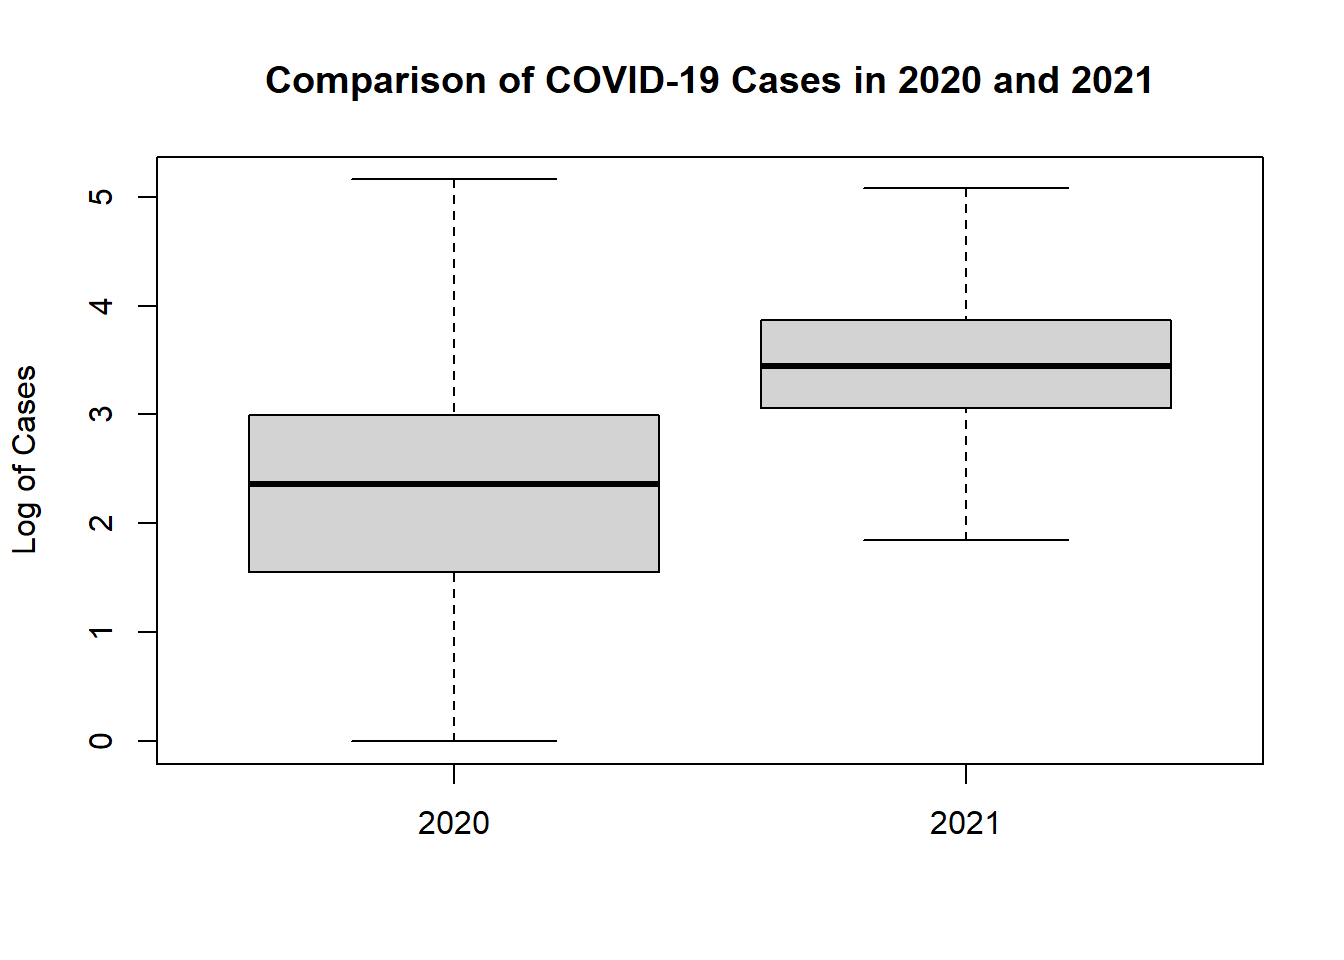
\includegraphics{Analyzing_Covid_Data_files/figure-latex/unnamed-chunk-4-1.pdf}

\begin{Shaded}
\begin{Highlighting}[]
\FunctionTok{create\_boxplot}\NormalTok{(Covid2020}\SpecialCharTok{$}\NormalTok{logdeaths, Covid2021}\SpecialCharTok{$}\NormalTok{logdeaths, }\StringTok{"Comparison of COVID{-}19 Deaths in 2020 and 2021"}\NormalTok{, }\StringTok{"Log of Deaths"}\NormalTok{)}
\end{Highlighting}
\end{Shaded}

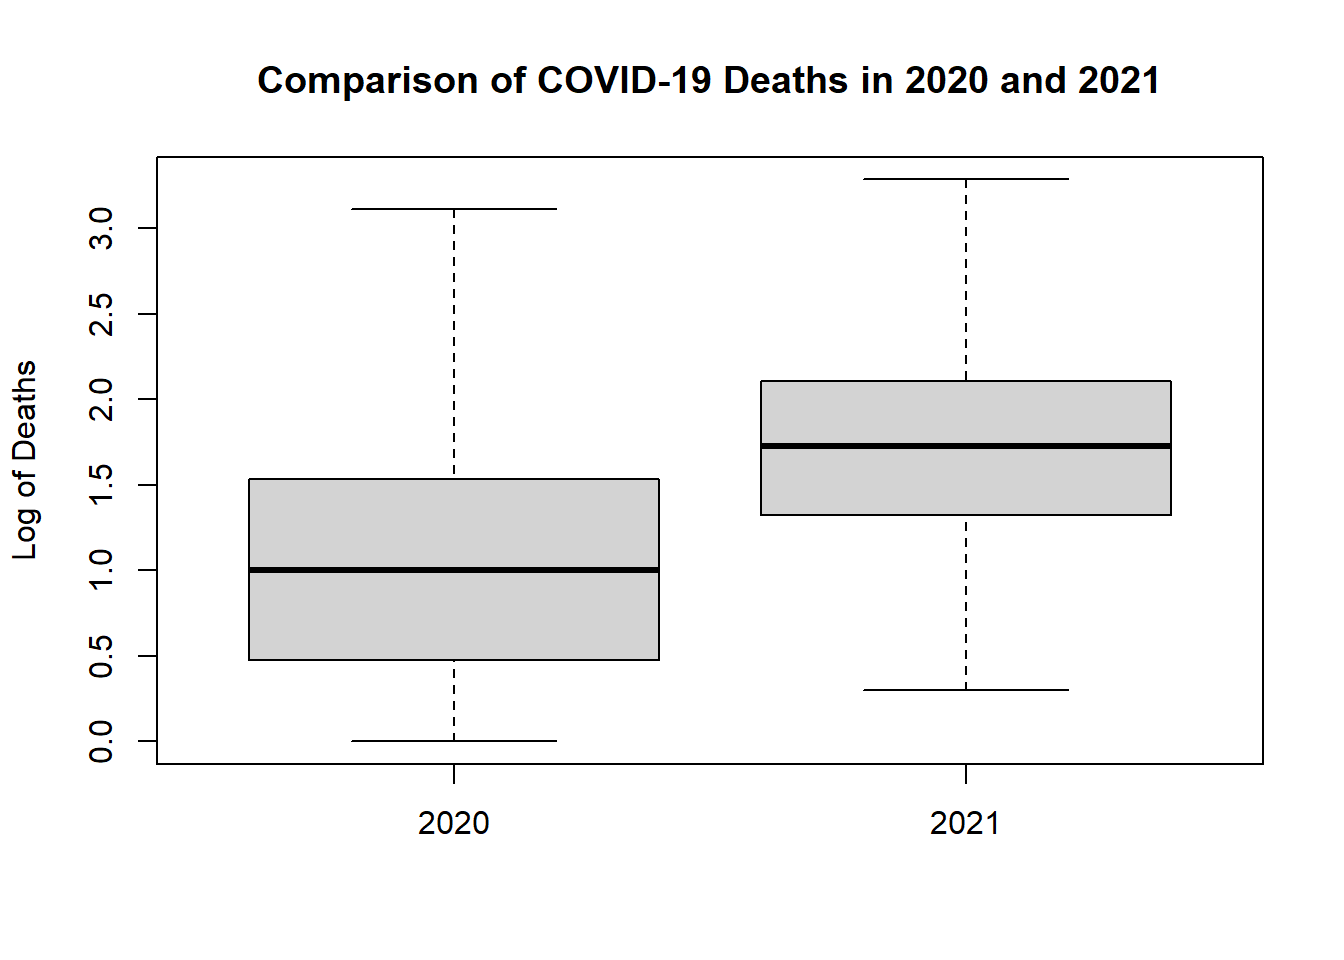
\includegraphics{Analyzing_Covid_Data_files/figure-latex/unnamed-chunk-4-2.pdf}
\emph{Capturing the summary of all original data along with the log data
to understand the above box plot better}

\begin{Shaded}
\begin{Highlighting}[]
\CommentTok{\# Summary statistics for Cases}
\FunctionTok{print}\NormalTok{(}\StringTok{"Summary 2020 cases"}\NormalTok{)}
\end{Highlighting}
\end{Shaded}

\begin{verbatim}
## [1] "Summary 2020 cases"
\end{verbatim}

\begin{Shaded}
\begin{Highlighting}[]
\FunctionTok{summary}\NormalTok{(Covid2020}\SpecialCharTok{$}\NormalTok{cases)}
\end{Highlighting}
\end{Shaded}

\begin{verbatim}
##    Min. 1st Qu.  Median    Mean 3rd Qu.    Max. 
##       0      36     228    1952     993  770915
\end{verbatim}

\begin{Shaded}
\begin{Highlighting}[]
\FunctionTok{summary}\NormalTok{(Covid2020}\SpecialCharTok{$}\NormalTok{logcases[Covid2020}\SpecialCharTok{$}\NormalTok{logcases}\SpecialCharTok{!={-}}\ConstantTok{Inf}\NormalTok{])}
\end{Highlighting}
\end{Shaded}

\begin{verbatim}
##    Min. 1st Qu.  Median    Mean 3rd Qu.    Max. 
##   0.000   1.556   2.358   2.267   2.997   5.887
\end{verbatim}

\begin{Shaded}
\begin{Highlighting}[]
\FunctionTok{print}\NormalTok{(}\StringTok{"Summary 2021 cases"}\NormalTok{)}
\end{Highlighting}
\end{Shaded}

\begin{verbatim}
## [1] "Summary 2021 cases"
\end{verbatim}

\begin{Shaded}
\begin{Highlighting}[]
\FunctionTok{summary}\NormalTok{(Covid2021}\SpecialCharTok{$}\NormalTok{cases)}
\end{Highlighting}
\end{Shaded}

\begin{verbatim}
##    Min. 1st Qu.  Median    Mean 3rd Qu.    Max. 
##       0    1136    2778   11160    7340 1697286
\end{verbatim}

\begin{Shaded}
\begin{Highlighting}[]
\FunctionTok{summary}\NormalTok{(Covid2021}\SpecialCharTok{$}\NormalTok{logcases[Covid2021}\SpecialCharTok{$}\NormalTok{logcases}\SpecialCharTok{!={-}}\ConstantTok{Inf}\NormalTok{])}
\end{Highlighting}
\end{Shaded}

\begin{verbatim}
##    Min. 1st Qu.  Median    Mean 3rd Qu.    Max. 
##   0.000   3.057   3.445   3.471   3.866   6.230
\end{verbatim}

\begin{Shaded}
\begin{Highlighting}[]
\CommentTok{\# Summary statistics for Deaths}
\FunctionTok{print}\NormalTok{(}\StringTok{"Summary 2020 Deaths"}\NormalTok{)}
\end{Highlighting}
\end{Shaded}

\begin{verbatim}
## [1] "Summary 2020 Deaths"
\end{verbatim}

\begin{Shaded}
\begin{Highlighting}[]
\FunctionTok{summary}\NormalTok{(Covid2020}\SpecialCharTok{$}\NormalTok{deaths)}
\end{Highlighting}
\end{Shaded}

\begin{verbatim}
##    Min. 1st Qu.  Median    Mean 3rd Qu.    Max.    NA's 
##     0.0     0.0     4.0    53.6    21.0 25144.0   18761
\end{verbatim}

\begin{Shaded}
\begin{Highlighting}[]
\FunctionTok{summary}\NormalTok{(Covid2020}\SpecialCharTok{$}\NormalTok{logdeaths[Covid2020}\SpecialCharTok{$}\NormalTok{logdeaths}\SpecialCharTok{!={-}}\ConstantTok{Inf}\NormalTok{])}
\end{Highlighting}
\end{Shaded}

\begin{verbatim}
##    Min. 1st Qu.  Median    Mean 3rd Qu.    Max.    NA's 
##   0.000   0.477   1.000   1.048   1.531   4.400   18761
\end{verbatim}

\begin{Shaded}
\begin{Highlighting}[]
\FunctionTok{print}\NormalTok{(}\StringTok{"Summary 2021 Deaths"}\NormalTok{)}
\end{Highlighting}
\end{Shaded}

\begin{verbatim}
## [1] "Summary 2021 Deaths"
\end{verbatim}

\begin{Shaded}
\begin{Highlighting}[]
\FunctionTok{summary}\NormalTok{(Covid2021}\SpecialCharTok{$}\NormalTok{deaths)}
\end{Highlighting}
\end{Shaded}

\begin{verbatim}
##    Min. 1st Qu.  Median    Mean 3rd Qu.    Max.    NA's 
##     0.0    20.0    52.0   193.6   125.0 35382.0   28470
\end{verbatim}

\begin{Shaded}
\begin{Highlighting}[]
\FunctionTok{summary}\NormalTok{(Covid2021}\SpecialCharTok{$}\NormalTok{logdeaths[Covid2021}\SpecialCharTok{$}\NormalTok{logdeaths}\SpecialCharTok{!={-}}\ConstantTok{Inf}\NormalTok{])}
\end{Highlighting}
\end{Shaded}

\begin{verbatim}
##    Min. 1st Qu.  Median    Mean 3rd Qu.    Max.    NA's 
##   0.000   1.322   1.724   1.731   2.107   4.549   28470
\end{verbatim}

\emph{The range of this dataset is very big. The minimum and maximum
value of the number of cases in 2020 are 0 and 770915 with a mean value
of 1952. The minimum and maximum value of the number of deaths in 2020
are 0 and 25144 with a mean value of 53.6.The minimum and maximum value
of the number of cases in 2021 are 0 and 1697286 with a mean value of
11160.The minimum and maximum value of the number of deaths in 2021 are
0 and 35382 with a mean value of 193.6.}

\emph{Plotting the number of covid cases and deaths for both 2020 and
2021 in each month to understand the data}

\begin{Shaded}
\begin{Highlighting}[]
\NormalTok{Covid2020}\SpecialCharTok{$}\NormalTok{date }\OtherTok{\textless{}{-}} \FunctionTok{as.Date}\NormalTok{(Covid2020}\SpecialCharTok{$}\NormalTok{date)}
\NormalTok{Covid2021}\SpecialCharTok{$}\NormalTok{date }\OtherTok{\textless{}{-}} \FunctionTok{as.Date}\NormalTok{(Covid2021}\SpecialCharTok{$}\NormalTok{date)}

\CommentTok{\# Summarize Cases for 2020 and 2021}
\NormalTok{cases\_by\_day\_2020 }\OtherTok{\textless{}{-}} \FunctionTok{summarize\_by\_day}\NormalTok{(Covid2020, cases)}
\NormalTok{cases\_by\_day\_2021 }\OtherTok{\textless{}{-}} \FunctionTok{summarize\_by\_day}\NormalTok{(Covid2021, cases)}

\CommentTok{\# Plot total cases by day for 2020 and 2021}
\FunctionTok{plot\_daily\_totals}\NormalTok{(cases\_by\_day\_2020, }\StringTok{"Total COVID{-}19 Cases by day (2020)"}\NormalTok{, }\StringTok{"Total Cases"}\NormalTok{, }\StringTok{"lightblue"}\NormalTok{)}
\end{Highlighting}
\end{Shaded}

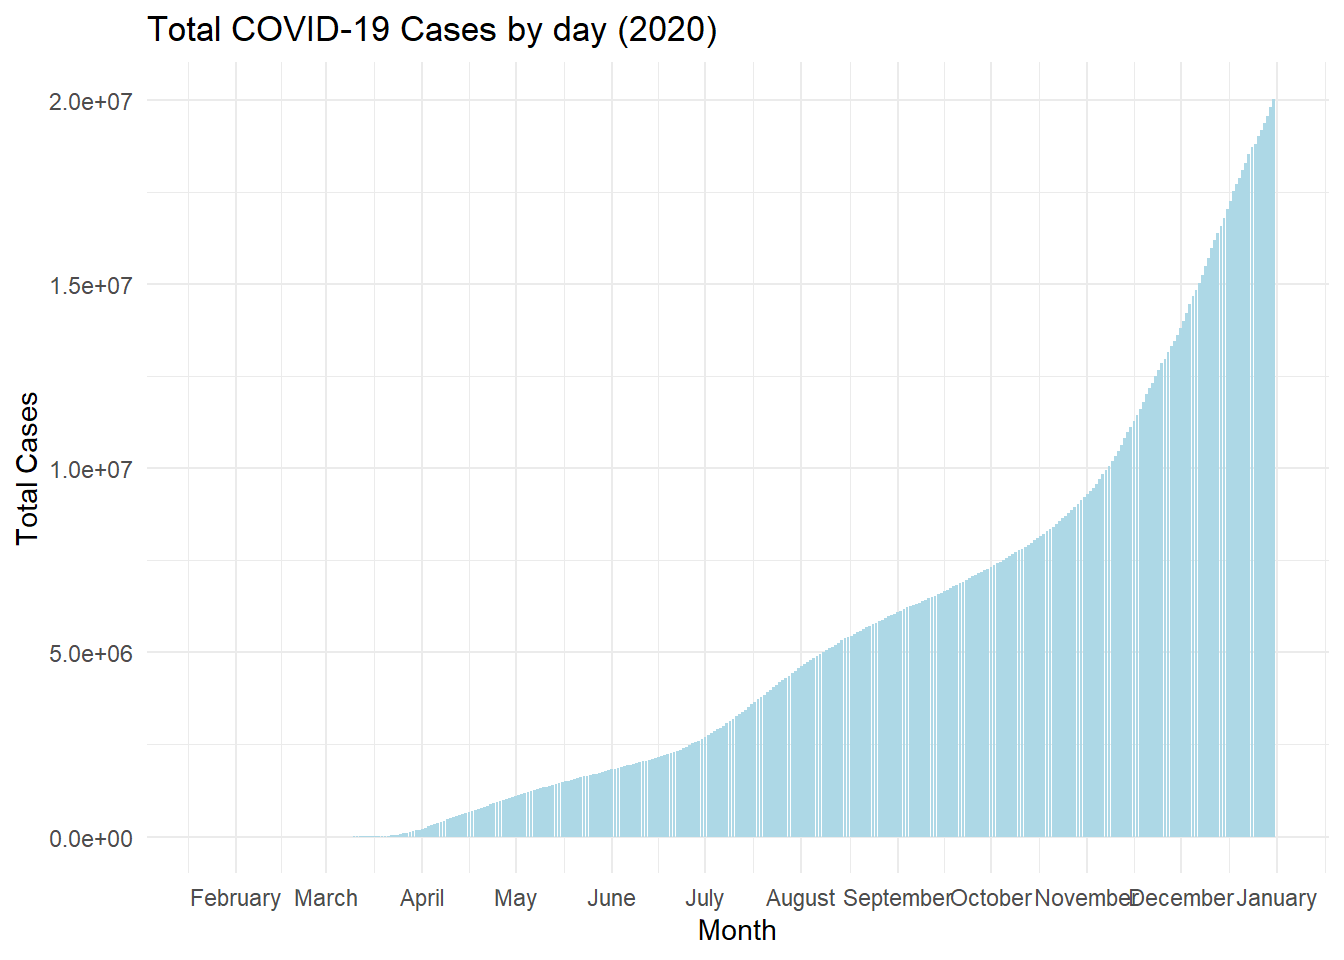
\includegraphics{Analyzing_Covid_Data_files/figure-latex/Number of cases in each month comparison-1.pdf}

\begin{Shaded}
\begin{Highlighting}[]
\FunctionTok{plot\_daily\_totals}\NormalTok{(cases\_by\_day\_2021, }\StringTok{"Total COVID{-}19 Cases by day (2021)"}\NormalTok{, }\StringTok{"Total Cases"}\NormalTok{, }\StringTok{"lightpink"}\NormalTok{)}
\end{Highlighting}
\end{Shaded}

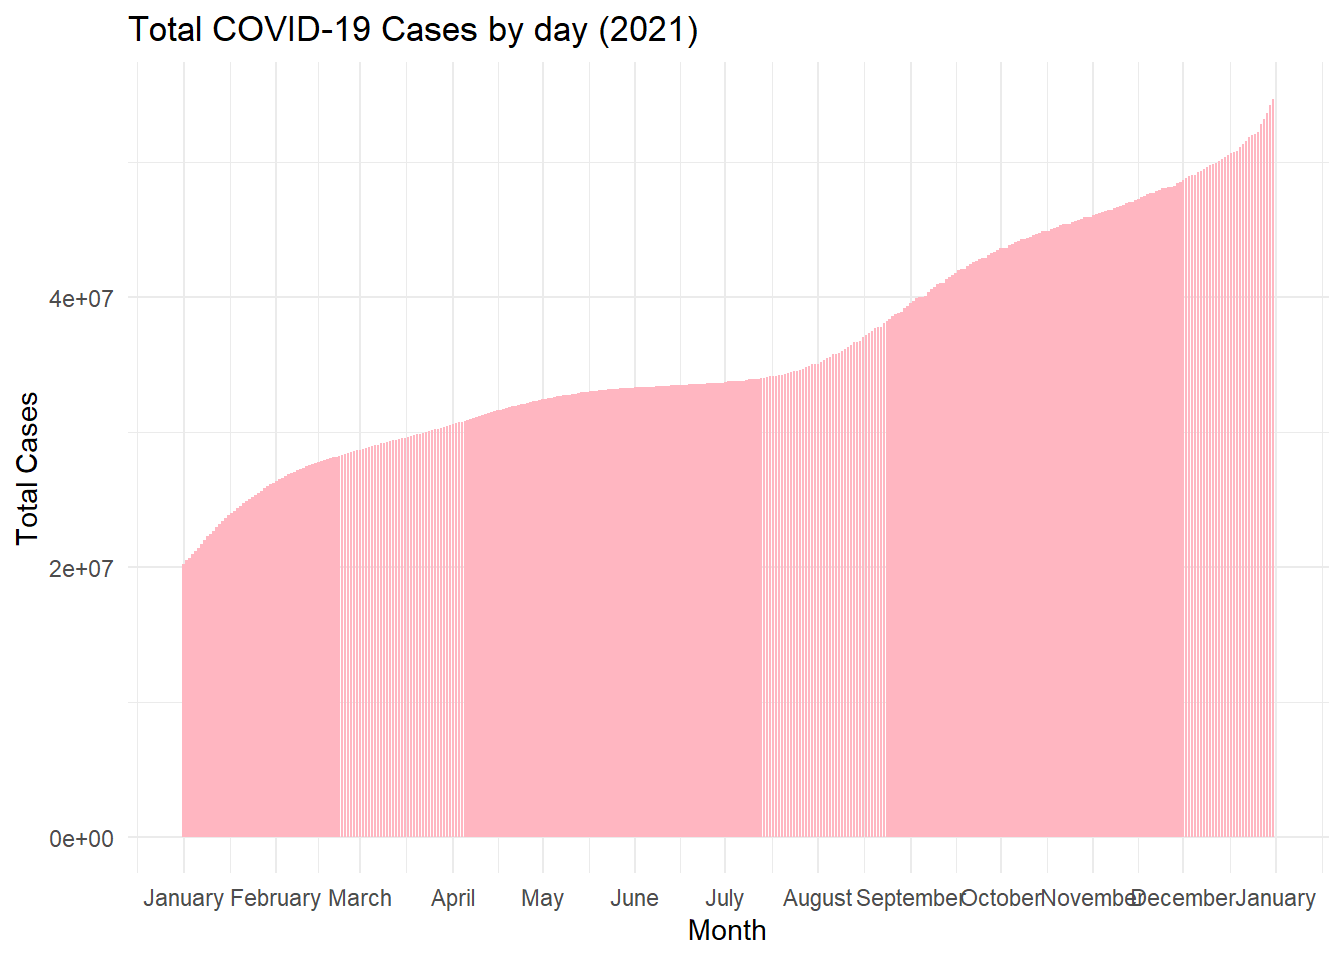
\includegraphics{Analyzing_Covid_Data_files/figure-latex/Number of cases in each month comparison-2.pdf}

\begin{Shaded}
\begin{Highlighting}[]
\CommentTok{\# Summarize deaths for 2020 and 2021}
\NormalTok{deaths\_by\_day\_2020 }\OtherTok{\textless{}{-}} \FunctionTok{summarize\_by\_day}\NormalTok{(Covid2020, deaths)}
\NormalTok{deaths\_by\_day\_2021 }\OtherTok{\textless{}{-}} \FunctionTok{summarize\_by\_day}\NormalTok{(Covid2021, deaths)}

\CommentTok{\# Plot total deaths by day for 2020 and 2021}
\FunctionTok{plot\_daily\_totals}\NormalTok{(deaths\_by\_day\_2020, }\StringTok{"Total COVID{-}19 Deaths by day (2020)"}\NormalTok{, }\StringTok{"Total Deaths"}\NormalTok{, }\StringTok{"darkblue"}\NormalTok{)}
\end{Highlighting}
\end{Shaded}

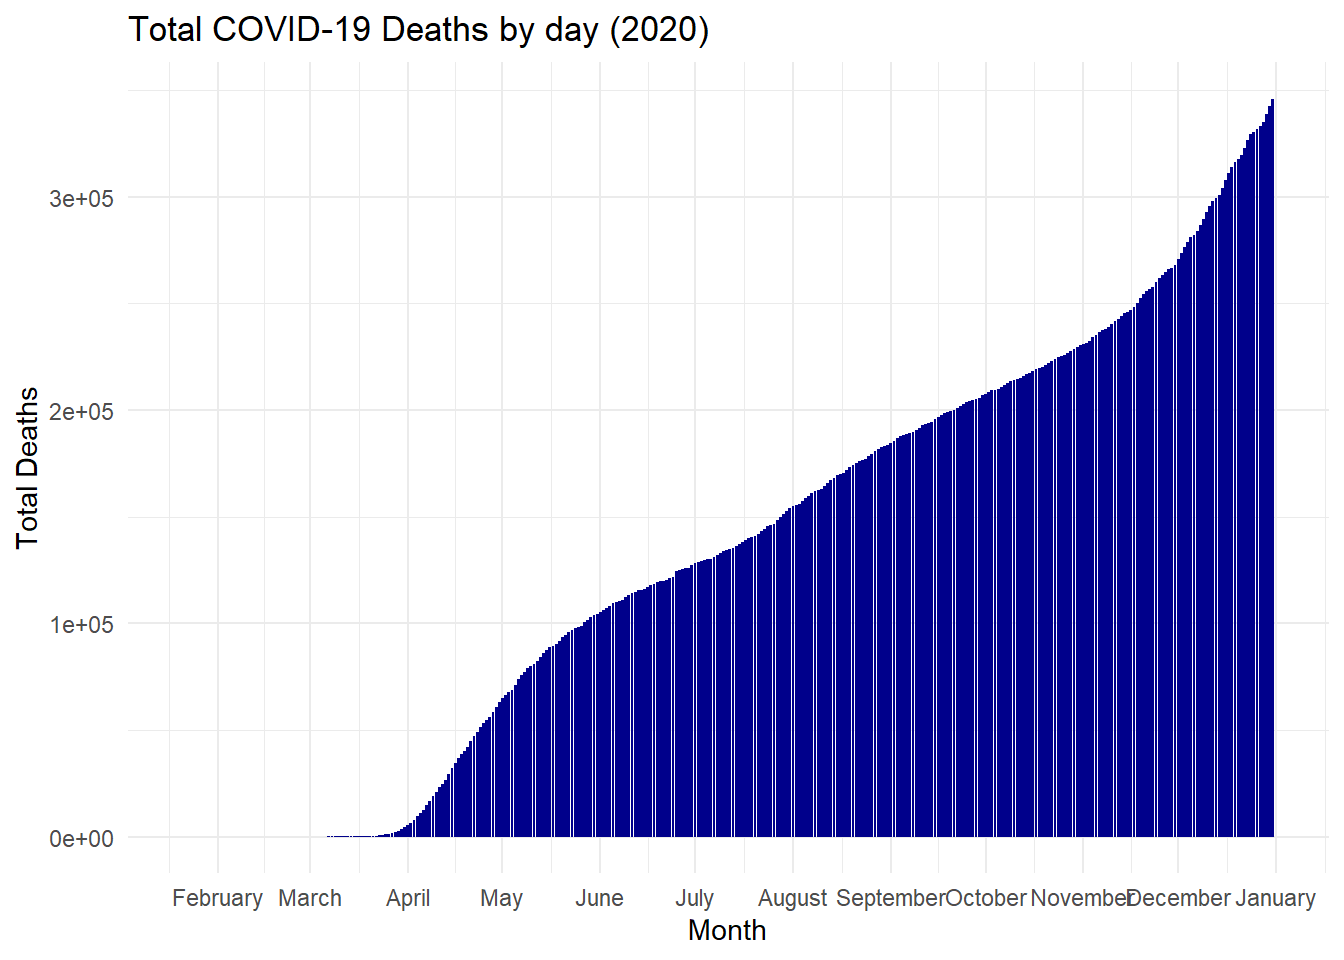
\includegraphics{Analyzing_Covid_Data_files/figure-latex/Number of cases in each month comparison-3.pdf}

\begin{Shaded}
\begin{Highlighting}[]
\FunctionTok{plot\_daily\_totals}\NormalTok{(deaths\_by\_day\_2021, }\StringTok{"Total COVID{-}19 Deaths by day (2021)"}\NormalTok{, }\StringTok{"Total Deaths"}\NormalTok{, }\StringTok{"darkgreen"}\NormalTok{)}
\end{Highlighting}
\end{Shaded}

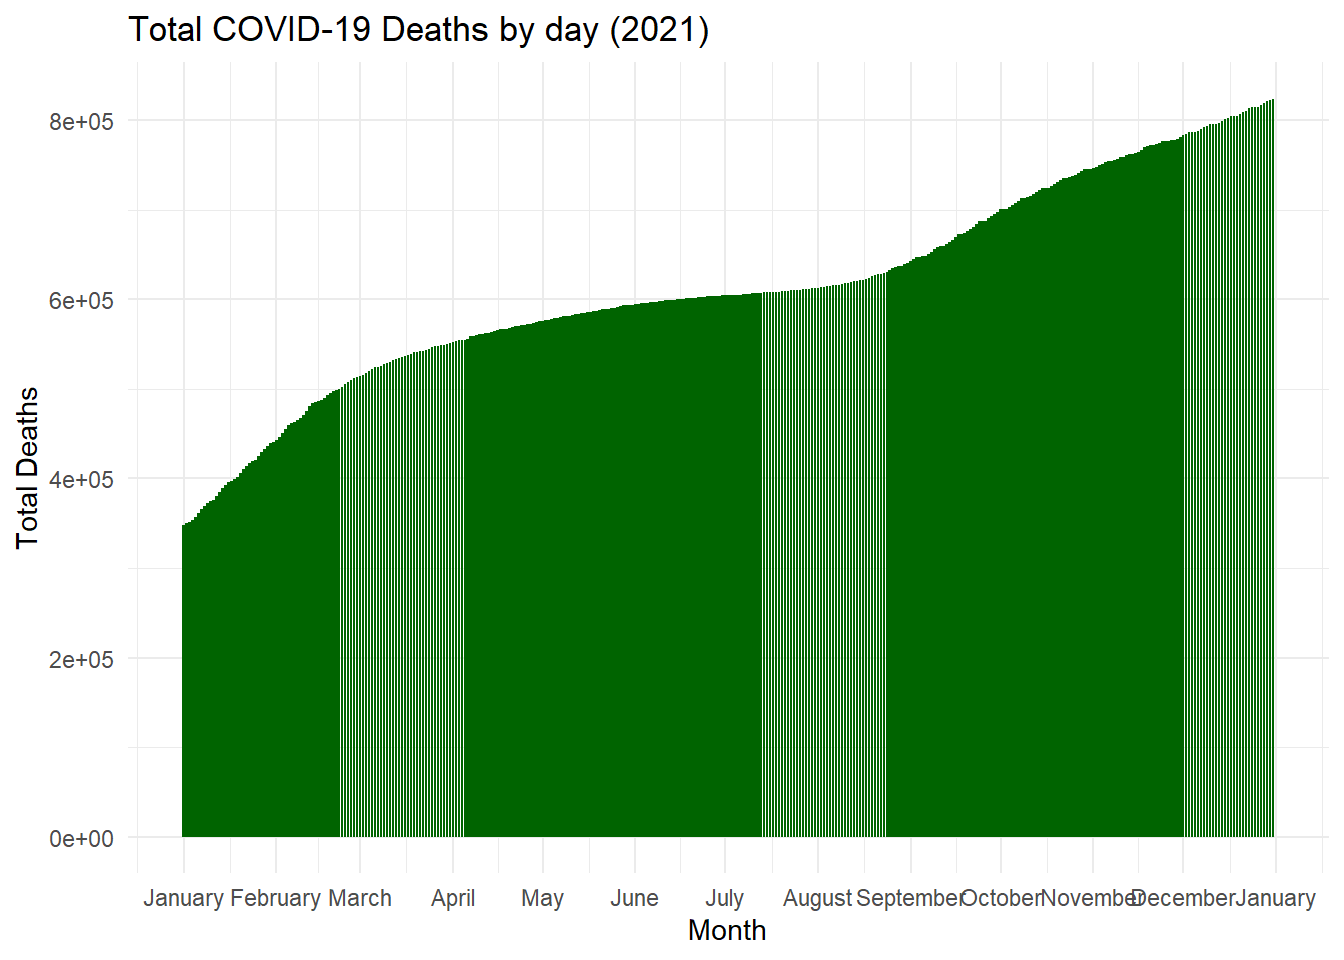
\includegraphics{Analyzing_Covid_Data_files/figure-latex/Number of cases in each month comparison-4.pdf}
\emph{The above graphs explains that the no of cases and deaths in both
the datasets for 2020 and 2021 are stored in cumulative format.} \#\#1 b

Create histograms for those two variables in the 2 datasets (you choose
the histogram bin width). Describe the distributions in terms of known
parametric distributions and similarities/ differences among them. Plot
the distribution you think matches the histogram (e.g.~normal,
chis-square, gamma, t-distribution, etc.) overlayed on the histogram.
min. 2-3 sentences

\emph{Analyzing 2020 data}

\begin{Shaded}
\begin{Highlighting}[]
\CommentTok{\# Filtering IQR for both cases and deaths for 2020}
\NormalTok{cases\_iqr\_2020 }\OtherTok{\textless{}{-}} \FunctionTok{filter\_iqr}\NormalTok{(Covid2020}\SpecialCharTok{$}\NormalTok{cases)}
\NormalTok{deaths\_iqr\_2020 }\OtherTok{\textless{}{-}} \FunctionTok{filter\_iqr}\NormalTok{(Covid2020}\SpecialCharTok{$}\NormalTok{deaths)}

\CommentTok{\# Remove non{-}positive values to capture a better graph}
\NormalTok{cases\_iqr\_2020 }\OtherTok{\textless{}{-}}\NormalTok{ cases\_iqr\_2020[cases\_iqr\_2020 }\SpecialCharTok{\textgreater{}} \DecValTok{0} \SpecialCharTok{\&} \SpecialCharTok{!}\FunctionTok{is.na}\NormalTok{(cases\_iqr\_2020) }\SpecialCharTok{\&} \FunctionTok{is.finite}\NormalTok{(cases\_iqr\_2020)]}
\NormalTok{deaths\_iqr\_2020 }\OtherTok{\textless{}{-}}\NormalTok{ deaths\_iqr\_2020[deaths\_iqr\_2020 }\SpecialCharTok{\textgreater{}} \DecValTok{0} \SpecialCharTok{\&} \SpecialCharTok{!}\FunctionTok{is.na}\NormalTok{(deaths\_iqr\_2020) }\SpecialCharTok{\&} \FunctionTok{is.finite}\NormalTok{(deaths\_iqr\_2020)]}

\CommentTok{\# Plot histogram and density for cases and deaths in 2020}
\FunctionTok{plot\_hist\_density}\NormalTok{(cases\_iqr\_2020, }\StringTok{"Histogram of COVID 2020 Cases with Density Overlay"}\NormalTok{, }\AttributeTok{binwidth =} \DecValTok{10}\NormalTok{)}
\end{Highlighting}
\end{Shaded}

\begin{verbatim}
## Warning: The dot-dot notation (`..density..`) was deprecated in ggplot2 3.4.0.
## i Please use `after_stat(density)` instead.
## This warning is displayed once every 8 hours.
## Call `lifecycle::last_lifecycle_warnings()` to see where this warning was
## generated.
\end{verbatim}

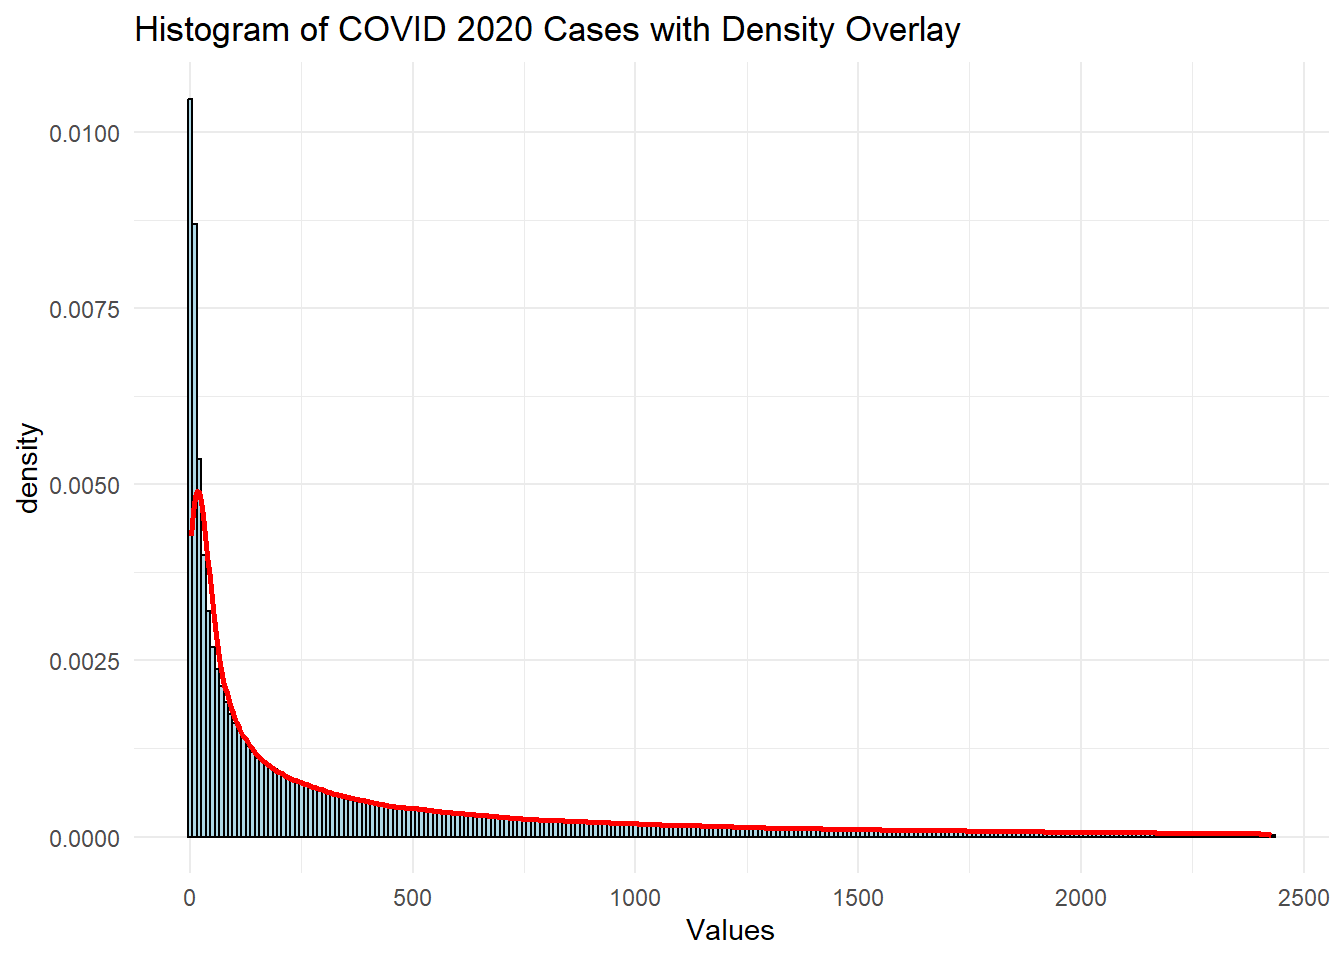
\includegraphics{Analyzing_Covid_Data_files/figure-latex/unnamed-chunk-6-1.pdf}

\begin{Shaded}
\begin{Highlighting}[]
\FunctionTok{plot\_hist\_density}\NormalTok{(deaths\_iqr\_2020, }\StringTok{"Histogram of COVID 2020 Deaths with Density Overlay"}\NormalTok{, }\AttributeTok{binwidth =} \DecValTok{1}\NormalTok{)}
\end{Highlighting}
\end{Shaded}

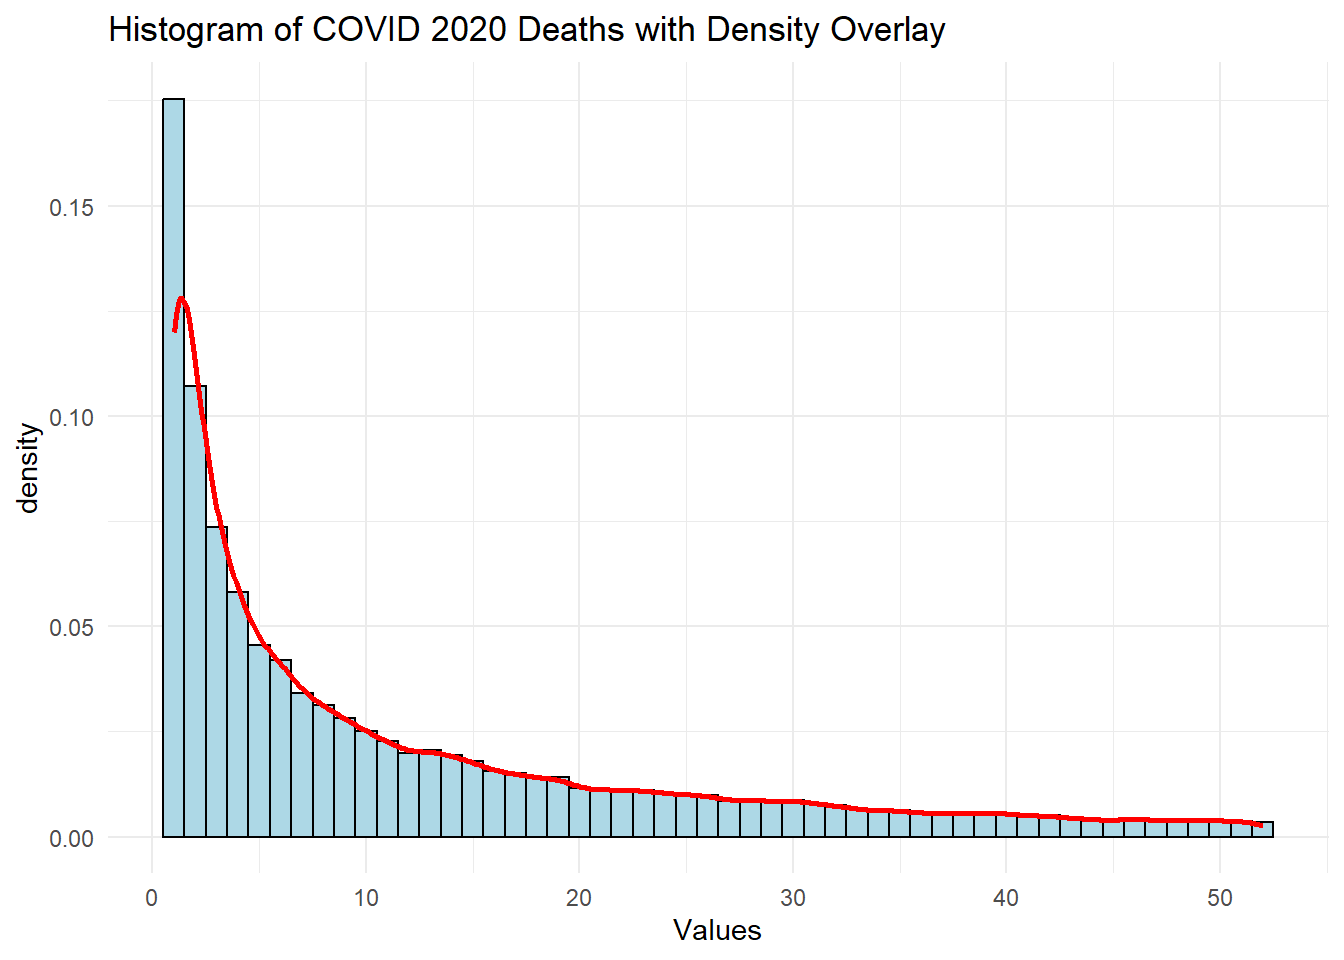
\includegraphics{Analyzing_Covid_Data_files/figure-latex/unnamed-chunk-6-2.pdf}
\emph{Since the data in both the above histograms are continuous,
positive and have skewed distribution. I think Gamma distribution would
be the best fit for both the graphs.}

\begin{Shaded}
\begin{Highlighting}[]
\FunctionTok{suppressWarnings}\NormalTok{(\{}
\FunctionTok{print}\NormalTok{(}\FunctionTok{plot\_gamma\_fit}\NormalTok{(cases\_iqr\_2020, }\StringTok{"Histogram of COVID Cases (IQR Filtered) with Gamma Distribution Overlay (2020)"}\NormalTok{, }\AttributeTok{binwidth =} \DecValTok{10}\NormalTok{))}

\FunctionTok{print}\NormalTok{(}\FunctionTok{plot\_gamma\_fit}\NormalTok{(deaths\_iqr\_2020, }\StringTok{"Histogram of COVID Deaths (IQR Filtered) with Gamma Distribution Overlay (2020)"}\NormalTok{, }\AttributeTok{binwidth =} \DecValTok{1}\NormalTok{))}
\NormalTok{\})}
\end{Highlighting}
\end{Shaded}

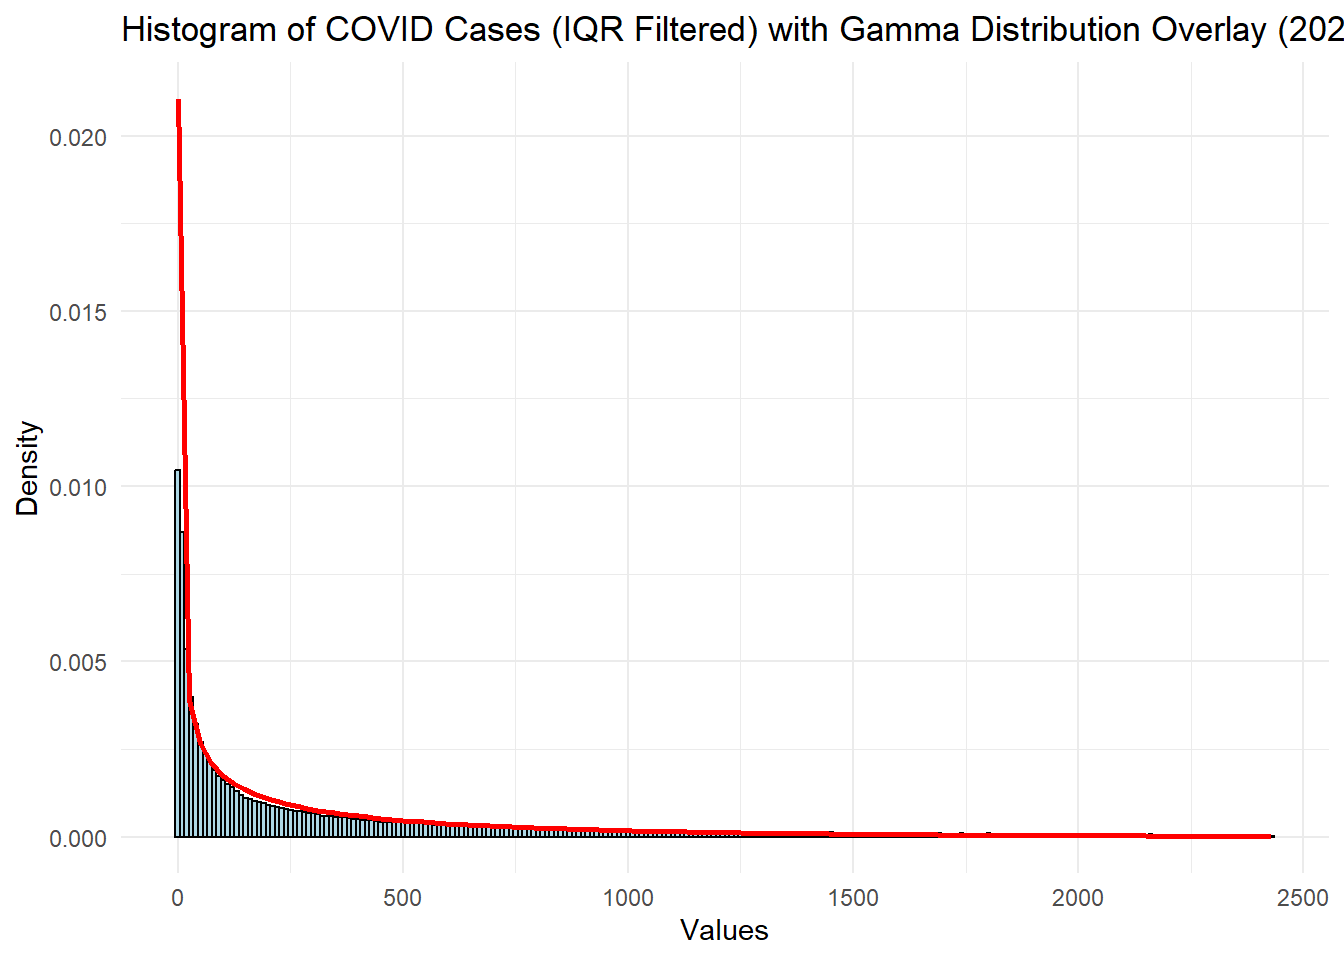
\includegraphics{Analyzing_Covid_Data_files/figure-latex/fitting gamma distribution in the cases plot 2020-1.pdf}
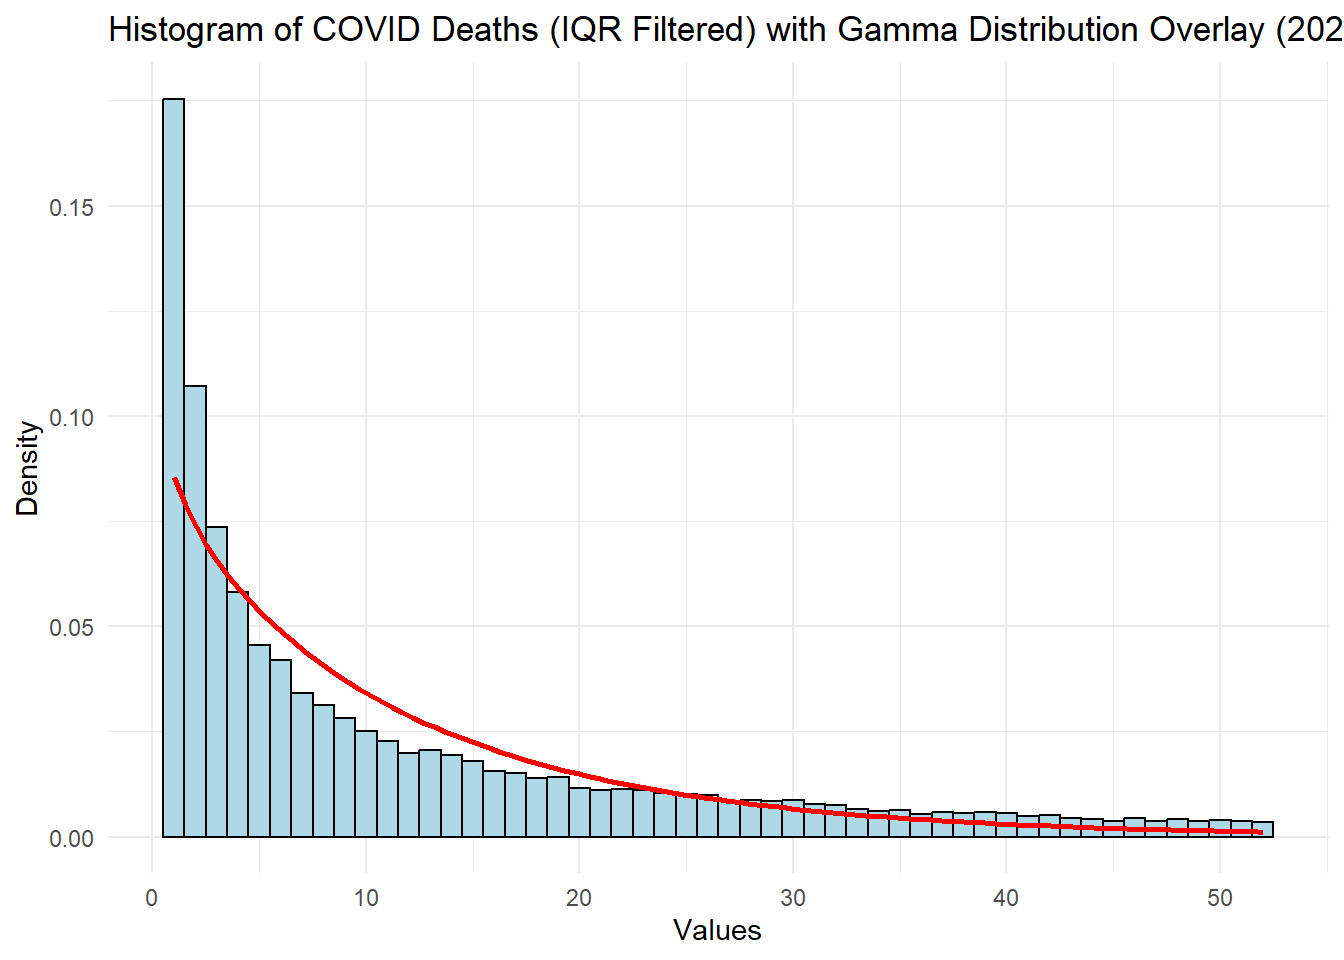
\includegraphics{Analyzing_Covid_Data_files/figure-latex/fitting gamma distribution in the cases plot 2020-2.pdf}

\emph{Analyzing 2021 data}

\begin{Shaded}
\begin{Highlighting}[]
\CommentTok{\# Repeat for 2021}
\NormalTok{cases\_iqr\_2021 }\OtherTok{\textless{}{-}} \FunctionTok{filter\_iqr}\NormalTok{(Covid2021}\SpecialCharTok{$}\NormalTok{cases)}
\NormalTok{deaths\_iqr\_2021 }\OtherTok{\textless{}{-}} \FunctionTok{filter\_iqr}\NormalTok{(Covid2021}\SpecialCharTok{$}\NormalTok{deaths)}

\CommentTok{\# Plot histogram and density for cases and deaths in 2021}
\FunctionTok{suppressWarnings}\NormalTok{(\{}
\FunctionTok{print}\NormalTok{(}\FunctionTok{plot\_hist\_density}\NormalTok{(cases\_iqr\_2021, }\StringTok{"Histogram of COVID 2021 Cases with Density Overlay"}\NormalTok{, }\AttributeTok{binwidth =} \DecValTok{100}\NormalTok{))}
\FunctionTok{print}\NormalTok{(}\FunctionTok{plot\_hist\_density}\NormalTok{(deaths\_iqr\_2021, }\StringTok{"Histogram of COVID 2021 Deaths with Density Overlay"}\NormalTok{, }\AttributeTok{binwidth =} \DecValTok{10}\NormalTok{))}
\NormalTok{\})}
\end{Highlighting}
\end{Shaded}

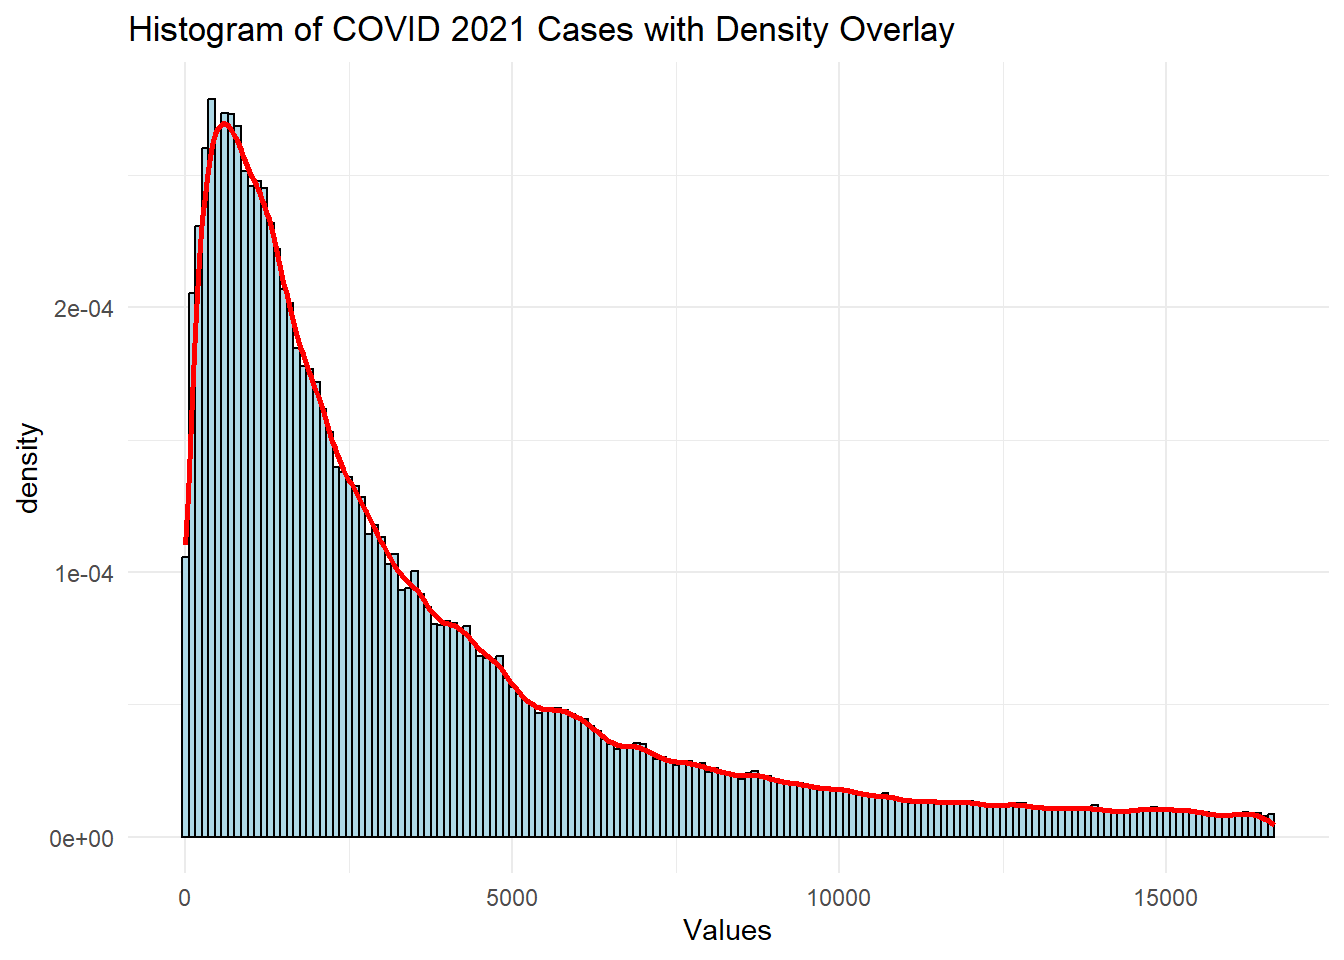
\includegraphics{Analyzing_Covid_Data_files/figure-latex/unnamed-chunk-7-1.pdf}
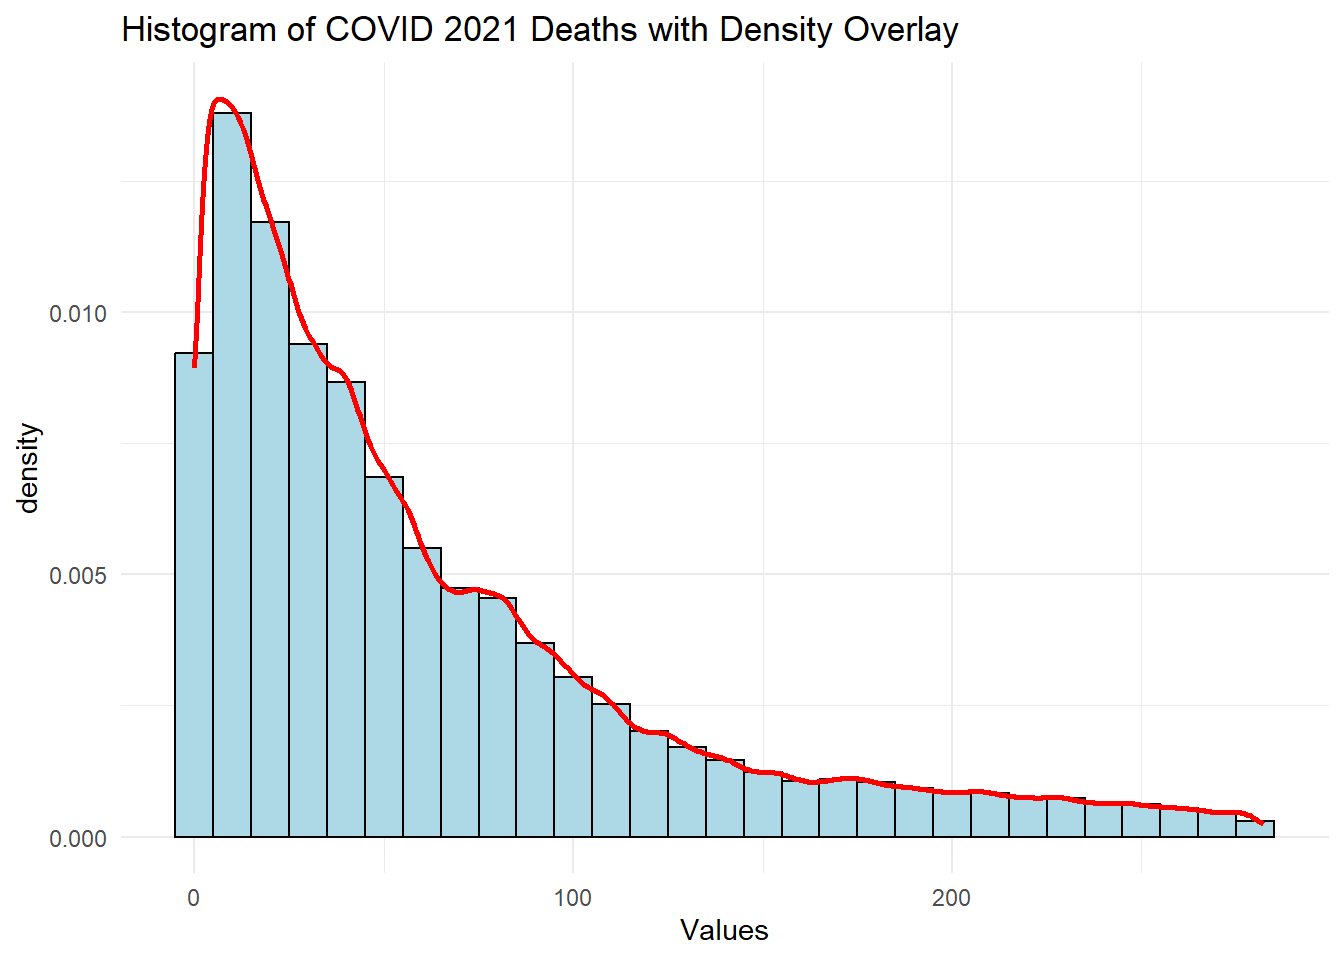
\includegraphics{Analyzing_Covid_Data_files/figure-latex/unnamed-chunk-7-2.pdf}
\emph{Similar to the 2020 data since the data in both the above
histograms are continuous, positive and have skewed distribution. I
think Gamma distribution would be the best fit for both the graphs.
Since the range of covid cases are very large the gamma fitting cannot
be done in the plot.}

\begin{Shaded}
\begin{Highlighting}[]
\CommentTok{\# Remove non{-}positive values and fit gamma distribution for 2021 cases and deaths}
\NormalTok{cases\_iqr\_2021 }\OtherTok{\textless{}{-}}\NormalTok{ cases\_iqr\_2021[cases\_iqr\_2021 }\SpecialCharTok{\textgreater{}} \DecValTok{0} \SpecialCharTok{\&} \SpecialCharTok{!}\FunctionTok{is.na}\NormalTok{(cases\_iqr\_2021) }\SpecialCharTok{\&} \FunctionTok{is.finite}\NormalTok{(cases\_iqr\_2021)]}
\NormalTok{deaths\_iqr\_2021 }\OtherTok{\textless{}{-}}\NormalTok{ deaths\_iqr\_2021[deaths\_iqr\_2021 }\SpecialCharTok{\textgreater{}} \DecValTok{0} \SpecialCharTok{\&} \SpecialCharTok{!}\FunctionTok{is.na}\NormalTok{(deaths\_iqr\_2021) }\SpecialCharTok{\&} \FunctionTok{is.finite}\NormalTok{(deaths\_iqr\_2021)]}
\FunctionTok{suppressWarnings}\NormalTok{(\{}
\CommentTok{\#plot\_gamma\_fit(cases\_iqr\_2021, "Histogram of COVID Cases (IQR Filtered) with Gamma Distribution Overlay (2021)", binwidth = 100)}
\FunctionTok{print}\NormalTok{(}\FunctionTok{plot\_gamma\_fit}\NormalTok{(deaths\_iqr\_2021, }\StringTok{"Histogram of COVID Deaths (IQR Filtered) with Gamma Distribution Overlay (2021)"}\NormalTok{, }\AttributeTok{binwidth =} \DecValTok{1}\NormalTok{))}
\NormalTok{\})}
\end{Highlighting}
\end{Shaded}

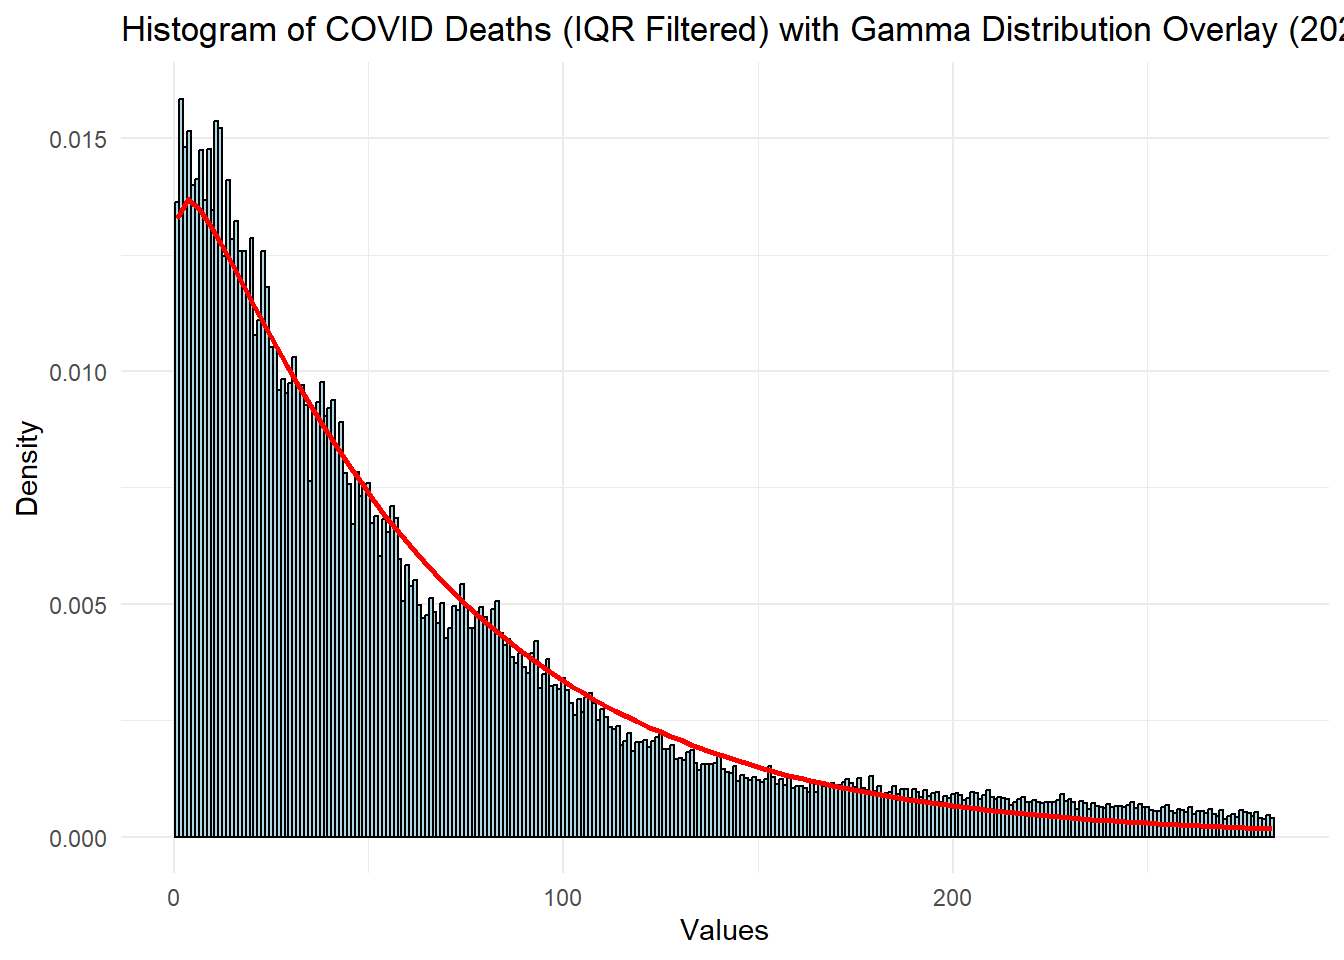
\includegraphics{Analyzing_Covid_Data_files/figure-latex/fitting gamma distribution in the cases plot 2021-1.pdf}
\textbf{Question 1 c } \emph{Plot the ECDFs (Empirical Cumulative
Distribution Function) for the two variables in both datasets. Plot the
quantile-quantile distribution using a suitable parametric distribution
you chose in 1b. Describe features of these plots. min. 2-3 sentences}

\begin{Shaded}
\begin{Highlighting}[]
\CommentTok{\# Plot ECDF for 2020 Cases and Deaths}

\FunctionTok{plot\_ecdf}\NormalTok{(cases\_by\_day\_2020}\SpecialCharTok{$}\NormalTok{total, }\StringTok{"ECDF of COVID 2020 Cases"}\NormalTok{, }\StringTok{"Cases"}\NormalTok{)}
\end{Highlighting}
\end{Shaded}

\includegraphics{Analyzing_Covid_Data_files/figure-latex/ECDF plots-1.pdf}

\begin{Shaded}
\begin{Highlighting}[]
\FunctionTok{plot\_ecdf}\NormalTok{(deaths\_by\_day\_2020}\SpecialCharTok{$}\NormalTok{total, }\StringTok{"ECDF of COVID 2020 Deaths"}\NormalTok{, }\StringTok{"Deaths"}\NormalTok{)}
\end{Highlighting}
\end{Shaded}

\includegraphics{Analyzing_Covid_Data_files/figure-latex/ECDF plots-2.pdf}

\begin{Shaded}
\begin{Highlighting}[]
\CommentTok{\# Plot ECDF for 2021 Cases and Deaths}
\FunctionTok{plot\_ecdf}\NormalTok{(cases\_by\_day\_2021}\SpecialCharTok{$}\NormalTok{total, }\StringTok{"ECDF of COVID 2021 Cases"}\NormalTok{, }\StringTok{"Cases"}\NormalTok{)}
\end{Highlighting}
\end{Shaded}

\includegraphics{Analyzing_Covid_Data_files/figure-latex/ECDF plots-3.pdf}

\begin{Shaded}
\begin{Highlighting}[]
\FunctionTok{plot\_ecdf}\NormalTok{(deaths\_by\_day\_2021}\SpecialCharTok{$}\NormalTok{total, }\StringTok{"ECDF of COVID 2021 Deaths"}\NormalTok{, }\StringTok{"Deaths"}\NormalTok{)}
\end{Highlighting}
\end{Shaded}

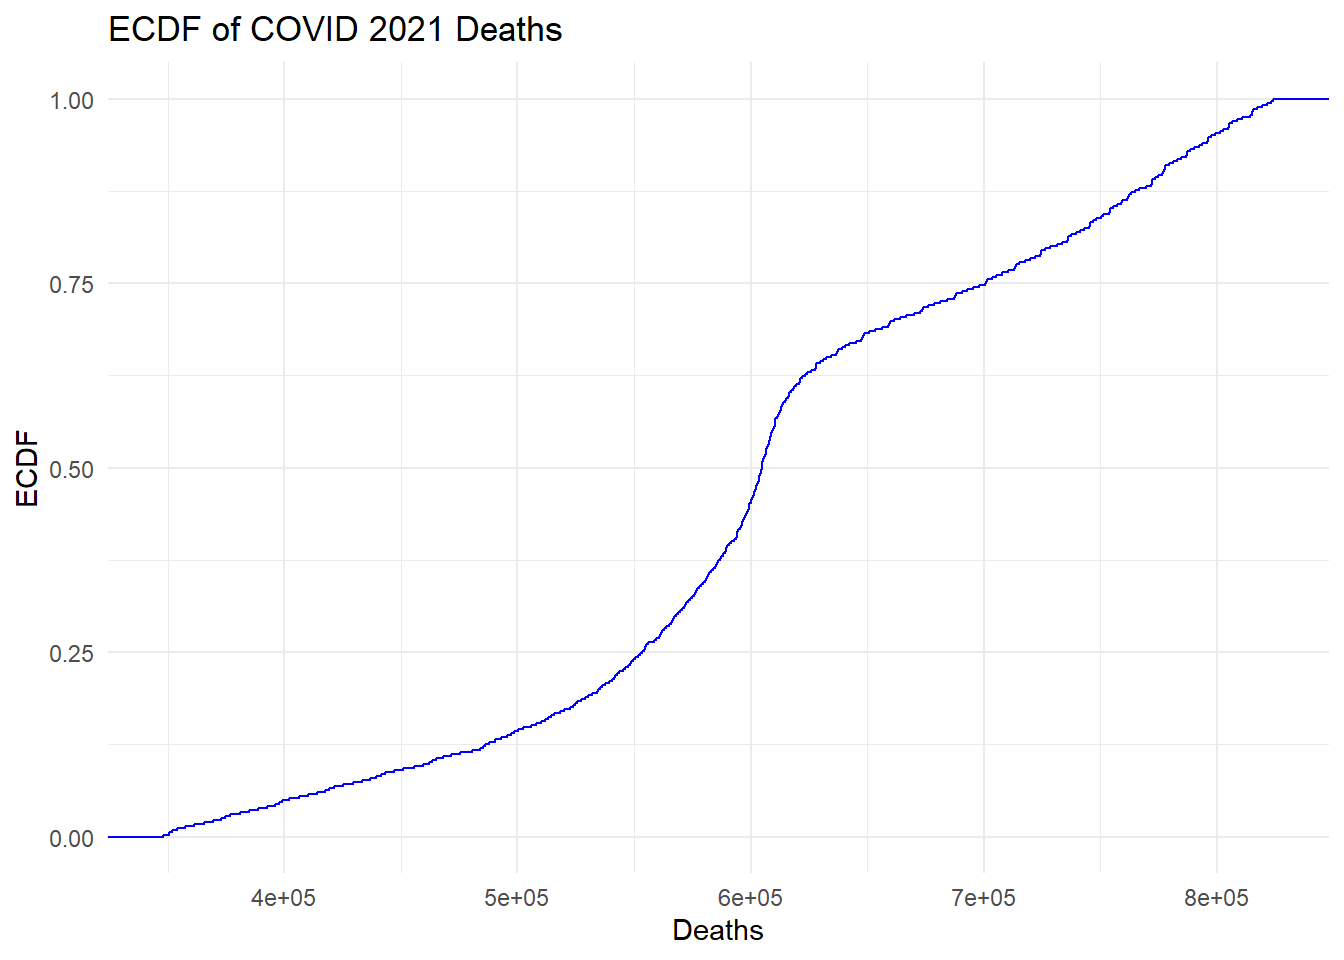
\includegraphics{Analyzing_Covid_Data_files/figure-latex/ECDF plots-4.pdf}
\emph{From the ECDF graph it is evident that in 2020 the total covid-19
cases was initially increasing slowly with a P-50 of around 3m. Later
from the second half of 2020 to 2021 the number of covid cases increased
faster. The 2021 graph has a comparatively gradual increase. }
\emph{There were very few deaths in the first quarter of the year. But
later through the remaining of 2020 and 2021, the number of deaths
gradually increased at a much faster rate. And, in the second half of
2021 the increase in death rate was much slower. }

\begin{Shaded}
\begin{Highlighting}[]
\FunctionTok{suppressWarnings}\NormalTok{(\{}
\CommentTok{\# Q{-}Q Plot against Gamma distribution for 2020 Cases and Deaths}
\FunctionTok{print}\NormalTok{(}\FunctionTok{plot\_qq\_gamma}\NormalTok{(cases\_iqr\_2020, }\StringTok{"Q{-}Q Plot of COVID 2020 Cases Against Fitted Gamma Distribution"}\NormalTok{))}
\FunctionTok{print}\NormalTok{(}\FunctionTok{plot\_qq\_gamma}\NormalTok{(deaths\_iqr\_2020, }\StringTok{"Q{-}Q Plot of COVID 2020 Deaths Against Fitted Gamma Distribution"}\NormalTok{))}

\CommentTok{\# Q{-}Q Plot against Gamma distribution for 2021 Cases and Deaths}
\CommentTok{\#print(plot\_qq\_gamma(cases\_iqr\_2021, "Q{-}Q Plot of COVID 2021 Cases Against Fitted Gamma Distribution"))}
\FunctionTok{print}\NormalTok{(}\FunctionTok{plot\_qq\_gamma}\NormalTok{(deaths\_iqr\_2021, }\StringTok{"Q{-}Q Plot of COVID 2021 Deaths Against Fitted Gamma Distribution"}\NormalTok{))}
\NormalTok{\})}
\end{Highlighting}
\end{Shaded}

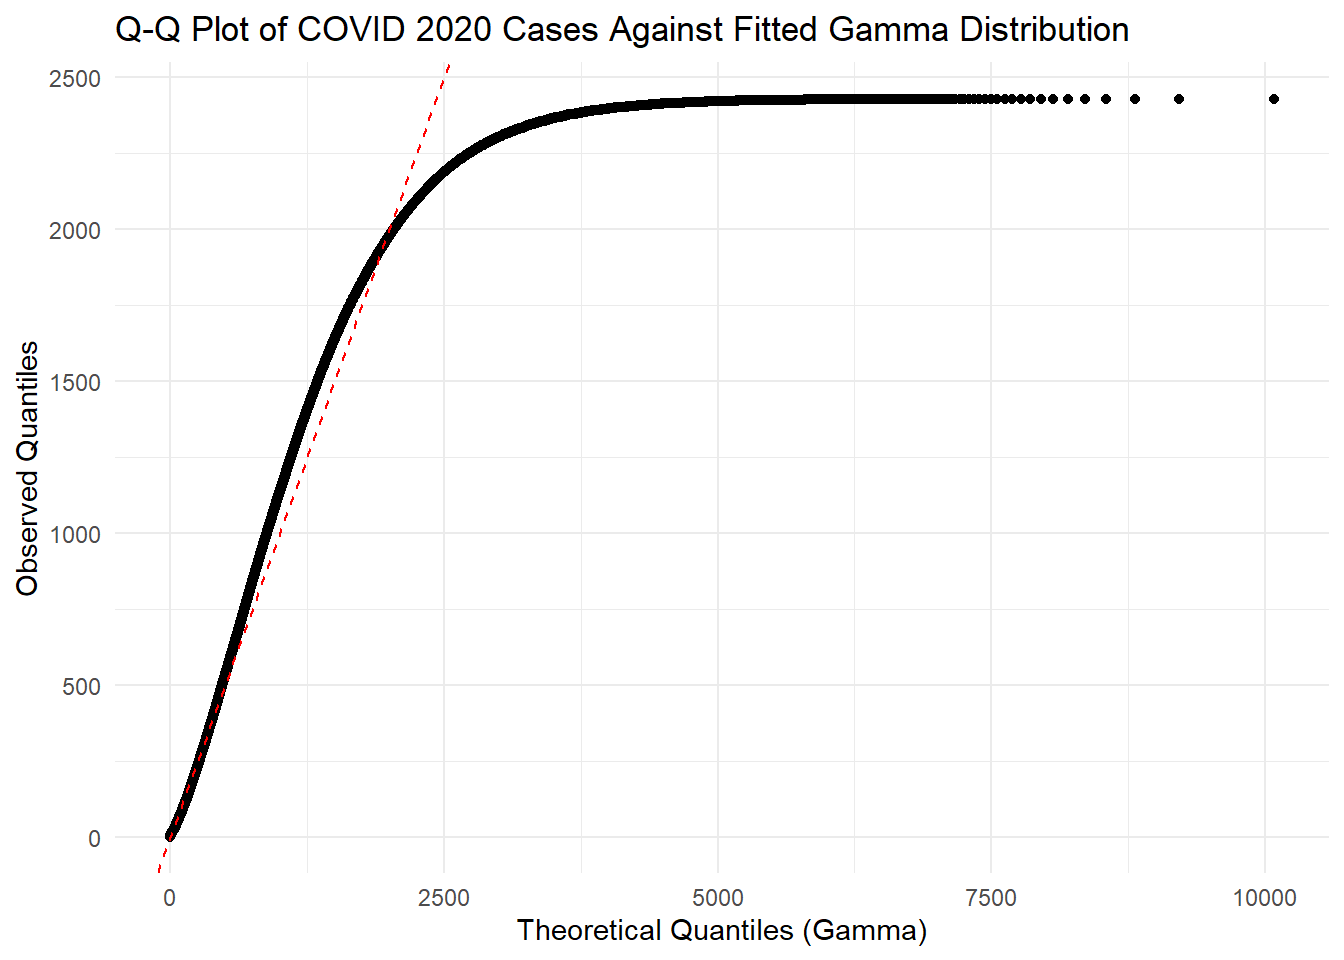
\includegraphics{Analyzing_Covid_Data_files/figure-latex/capturing all the QQ plot-1.pdf}
\includegraphics{Analyzing_Covid_Data_files/figure-latex/capturing all the QQ plot-2.pdf}
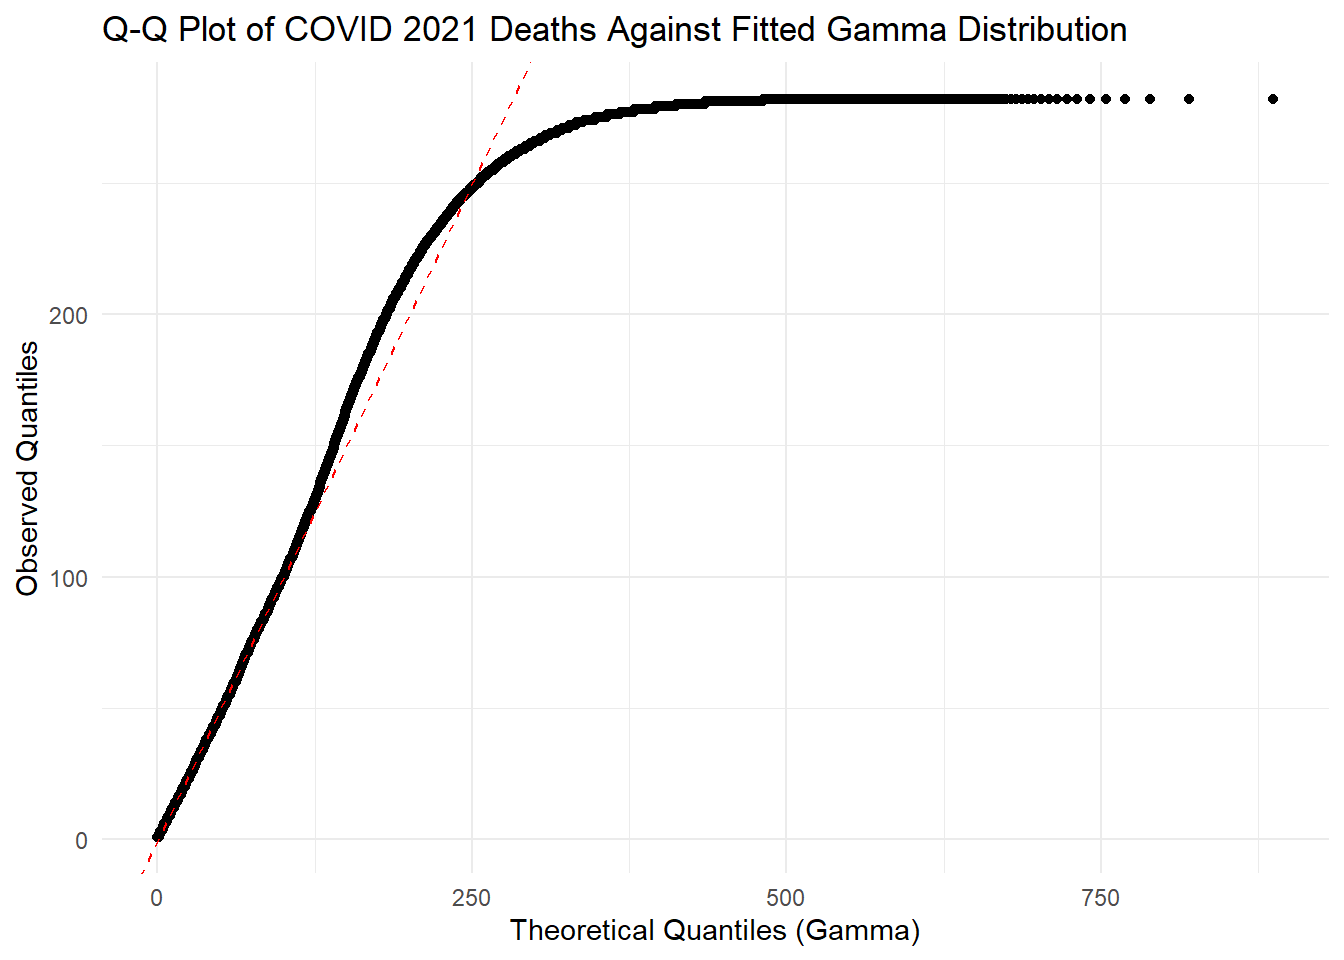
\includegraphics{Analyzing_Covid_Data_files/figure-latex/capturing all the QQ plot-3.pdf}
\emph{The above graphs explain that till a certain value in all the
graphs both the theoretical(values generated from the model) and
observed value are same. But later there is a sudden increase in the
theoritical value, and a large change is observed.}

\#\#1 c Filter the distributions you explored in Q1 by a number of
states or counties. Repeat Q1b, Q1c and Q1d and draw any conclusions
from this study. min. 3-4 sentences

\begin{Shaded}
\begin{Highlighting}[]
\CommentTok{\# Filter data for specific states}
\NormalTok{states }\OtherTok{\textless{}{-}} \FunctionTok{c}\NormalTok{(}\StringTok{"New York"}\NormalTok{, }\StringTok{"Washington"}\NormalTok{, }\StringTok{"Illinois"}\NormalTok{, }\StringTok{"California"}\NormalTok{)}
\NormalTok{Covid2020StateFiltered }\OtherTok{\textless{}{-}} \FunctionTok{filter\_by\_state}\NormalTok{(Covid2020, states)}
\NormalTok{Covid2021StateFiltered }\OtherTok{\textless{}{-}} \FunctionTok{filter\_by\_state}\NormalTok{(Covid2021, states)}

\CommentTok{\# Create boxplots comparing 2020 and 2021 for cases and deaths}
\FunctionTok{create\_boxplot}\NormalTok{(Covid2020StateFiltered}\SpecialCharTok{$}\NormalTok{logcases, Covid2021StateFiltered}\SpecialCharTok{$}\NormalTok{logcases, }\StringTok{"Comparison of COVID{-}19 Cases in 2020 and 2021"}\NormalTok{, }\StringTok{"Log of Cases"}\NormalTok{)}
\end{Highlighting}
\end{Shaded}

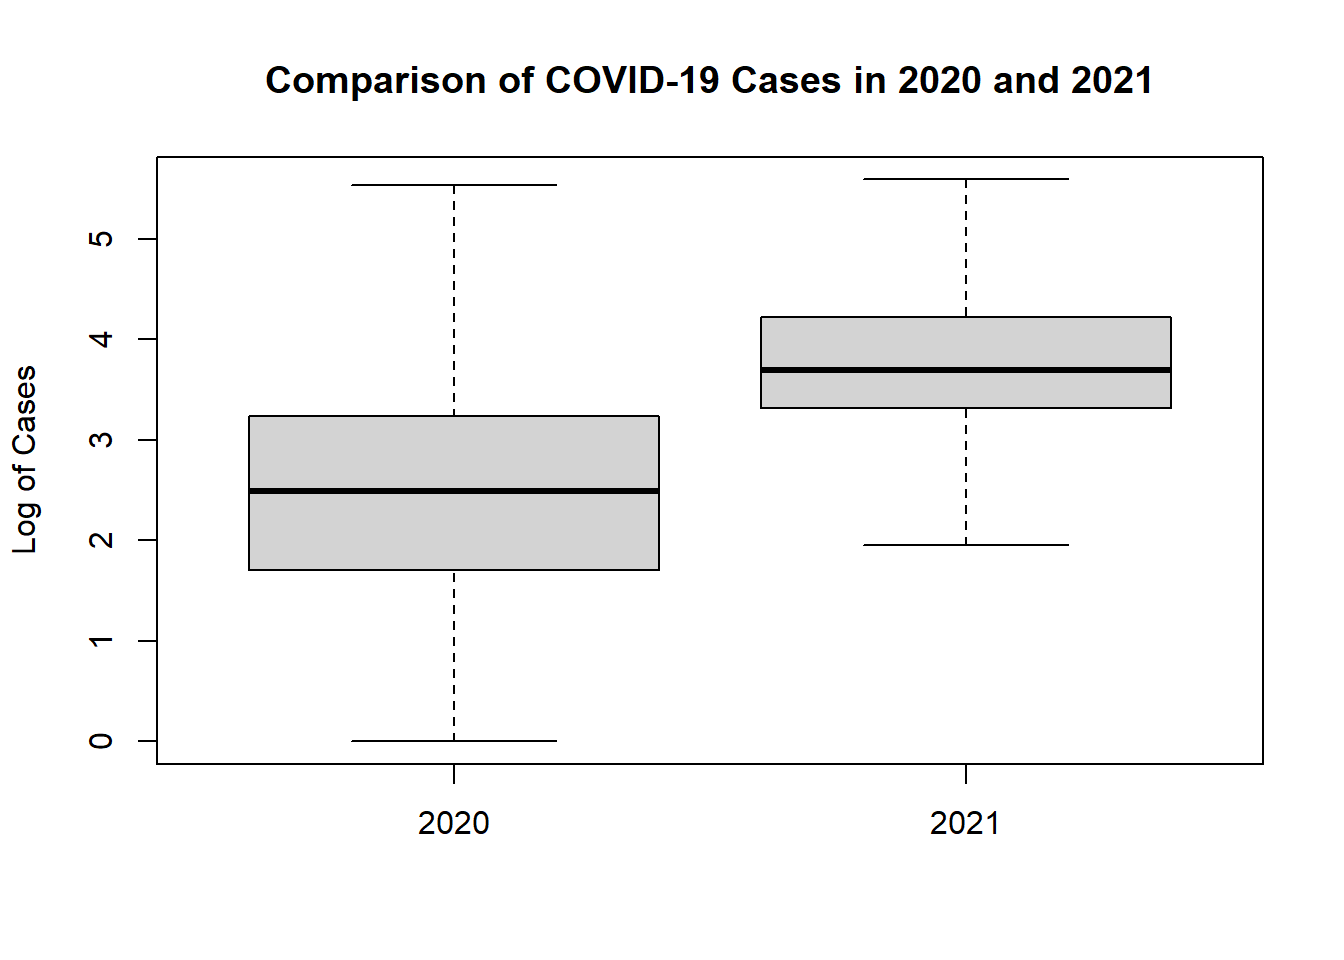
\includegraphics{Analyzing_Covid_Data_files/figure-latex/unnamed-chunk-8-1.pdf}

\begin{Shaded}
\begin{Highlighting}[]
\FunctionTok{create\_boxplot}\NormalTok{(Covid2020StateFiltered}\SpecialCharTok{$}\NormalTok{logdeaths, Covid2021StateFiltered}\SpecialCharTok{$}\NormalTok{logdeaths, }\StringTok{"Comparison of COVID{-}19 Deaths in 2020 and 2021"}\NormalTok{, }\StringTok{"Log of Deaths"}\NormalTok{)}
\end{Highlighting}
\end{Shaded}

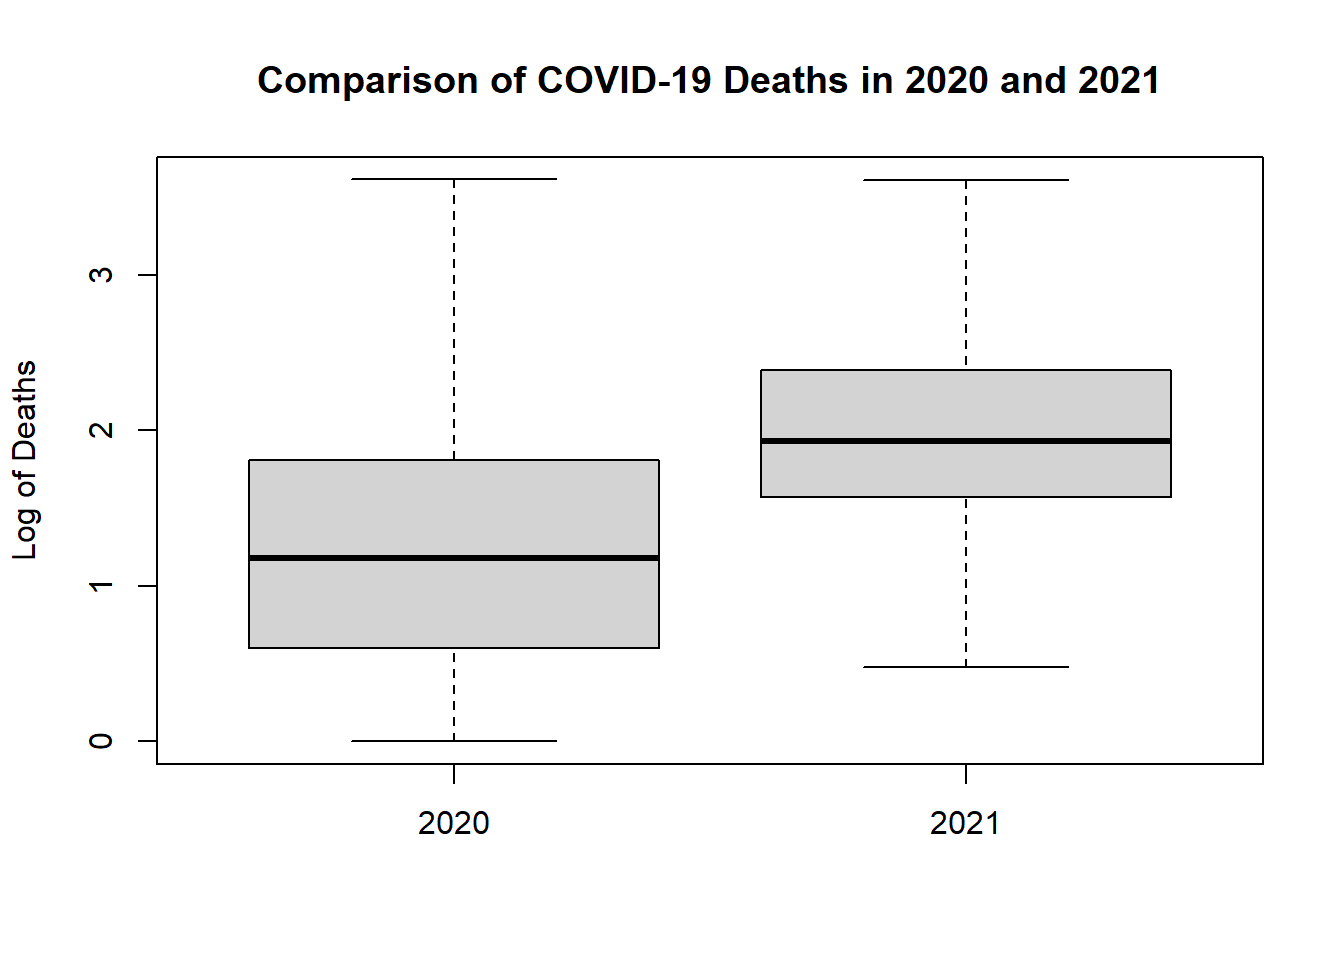
\includegraphics{Analyzing_Covid_Data_files/figure-latex/unnamed-chunk-8-2.pdf}

\begin{Shaded}
\begin{Highlighting}[]
\FunctionTok{summary}\NormalTok{(Covid2020StateFiltered}\SpecialCharTok{$}\NormalTok{cases)}
\end{Highlighting}
\end{Shaded}

\begin{verbatim}
##    Min. 1st Qu.  Median    Mean 3rd Qu.    Max. 
##       0      51     308    5529    1742  770915
\end{verbatim}

\begin{Shaded}
\begin{Highlighting}[]
\FunctionTok{summary}\NormalTok{(Covid2020StateFiltered}\SpecialCharTok{$}\NormalTok{logcases[Covid2020StateFiltered}\SpecialCharTok{$}\NormalTok{logcases}\SpecialCharTok{!={-}}\ConstantTok{Inf}\NormalTok{])}
\end{Highlighting}
\end{Shaded}

\begin{verbatim}
##    Min. 1st Qu.  Median    Mean 3rd Qu.    Max. 
##   0.000   1.708   2.489   2.469   3.241   5.887
\end{verbatim}

\begin{Shaded}
\begin{Highlighting}[]
\FunctionTok{summary}\NormalTok{(Covid2021StateFiltered}\SpecialCharTok{$}\NormalTok{cases)}
\end{Highlighting}
\end{Shaded}

\begin{verbatim}
##    Min. 1st Qu.  Median    Mean 3rd Qu.    Max. 
##       0    2052    4945   31712   16772 1697286
\end{verbatim}

\begin{Shaded}
\begin{Highlighting}[]
\FunctionTok{summary}\NormalTok{(Covid2021StateFiltered}\SpecialCharTok{$}\NormalTok{logcases[Covid2021StateFiltered}\SpecialCharTok{$}\NormalTok{logcases}\SpecialCharTok{!={-}}\ConstantTok{Inf}\NormalTok{])}
\end{Highlighting}
\end{Shaded}

\begin{verbatim}
##    Min. 1st Qu.  Median    Mean 3rd Qu.    Max. 
##   1.415   3.317   3.697   3.784   4.228   6.230
\end{verbatim}

\begin{Shaded}
\begin{Highlighting}[]
\FunctionTok{summary}\NormalTok{(Covid2020StateFiltered}\SpecialCharTok{$}\NormalTok{deaths)}
\end{Highlighting}
\end{Shaded}

\begin{verbatim}
##    Min. 1st Qu.  Median    Mean 3rd Qu.    Max. 
##     0.0     1.0     6.0   192.4    38.0 25144.0
\end{verbatim}

\begin{Shaded}
\begin{Highlighting}[]
\FunctionTok{summary}\NormalTok{(Covid2020StateFiltered}\SpecialCharTok{$}\NormalTok{logdeaths[Covid2020StateFiltered}\SpecialCharTok{$}\NormalTok{logdeaths}\SpecialCharTok{!={-}}\ConstantTok{Inf}\NormalTok{])}
\end{Highlighting}
\end{Shaded}

\begin{verbatim}
##    Min. 1st Qu.  Median    Mean 3rd Qu.    Max. 
##  0.0000  0.6021  1.1761  1.2550  1.8062  4.4004
\end{verbatim}

\begin{Shaded}
\begin{Highlighting}[]
\FunctionTok{summary}\NormalTok{(Covid2021StateFiltered}\SpecialCharTok{$}\NormalTok{deaths)}
\end{Highlighting}
\end{Shaded}

\begin{verbatim}
##    Min. 1st Qu.  Median    Mean 3rd Qu.    Max. 
##     0.0    36.0    83.0   564.2   236.0 35382.0
\end{verbatim}

\begin{Shaded}
\begin{Highlighting}[]
\FunctionTok{summary}\NormalTok{(Covid2021StateFiltered}\SpecialCharTok{$}\NormalTok{logdeaths[Covid2021StateFiltered}\SpecialCharTok{$}\NormalTok{logdeaths}\SpecialCharTok{!={-}}\ConstantTok{Inf}\NormalTok{])}
\end{Highlighting}
\end{Shaded}

\begin{verbatim}
##    Min. 1st Qu.  Median    Mean 3rd Qu.    Max. 
##   0.000   1.568   1.929   1.983   2.384   4.549
\end{verbatim}

\begin{Shaded}
\begin{Highlighting}[]
\CommentTok{\# Summarize Cases for 2020 and 2021}
\NormalTok{cases\_by\_day\_2020\_new }\OtherTok{\textless{}{-}} \FunctionTok{summarize\_by\_day}\NormalTok{(Covid2020StateFiltered, cases)}
\NormalTok{cases\_by\_day\_2021\_new }\OtherTok{\textless{}{-}} \FunctionTok{summarize\_by\_day}\NormalTok{(Covid2021StateFiltered, cases)}

\CommentTok{\# Plot total cases by day for 2020 and 2021}
\FunctionTok{plot\_daily\_totals}\NormalTok{(cases\_by\_day\_2020\_new, }\StringTok{"Total COVID{-}19 Cases by day (2020)"}\NormalTok{, }\StringTok{"Total Cases"}\NormalTok{, }\StringTok{"lightblue"}\NormalTok{)}
\end{Highlighting}
\end{Shaded}

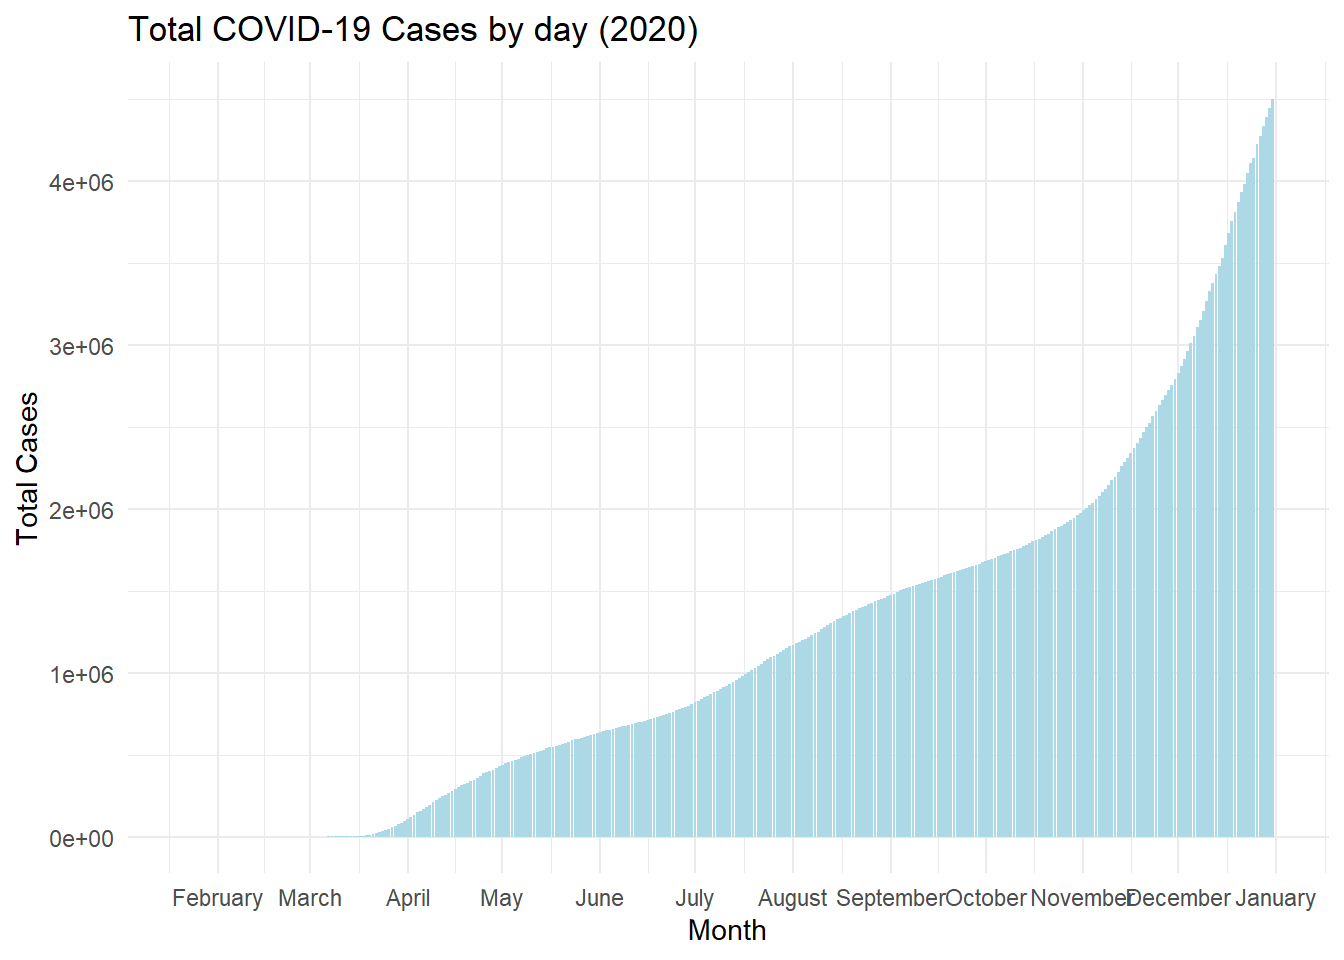
\includegraphics{Analyzing_Covid_Data_files/figure-latex/unnamed-chunk-8-3.pdf}

\begin{Shaded}
\begin{Highlighting}[]
\FunctionTok{plot\_daily\_totals}\NormalTok{(cases\_by\_day\_2021\_new, }\StringTok{"Total COVID{-}19 Cases by day (2021)"}\NormalTok{, }\StringTok{"Total Cases"}\NormalTok{, }\StringTok{"lightpink"}\NormalTok{)}
\end{Highlighting}
\end{Shaded}

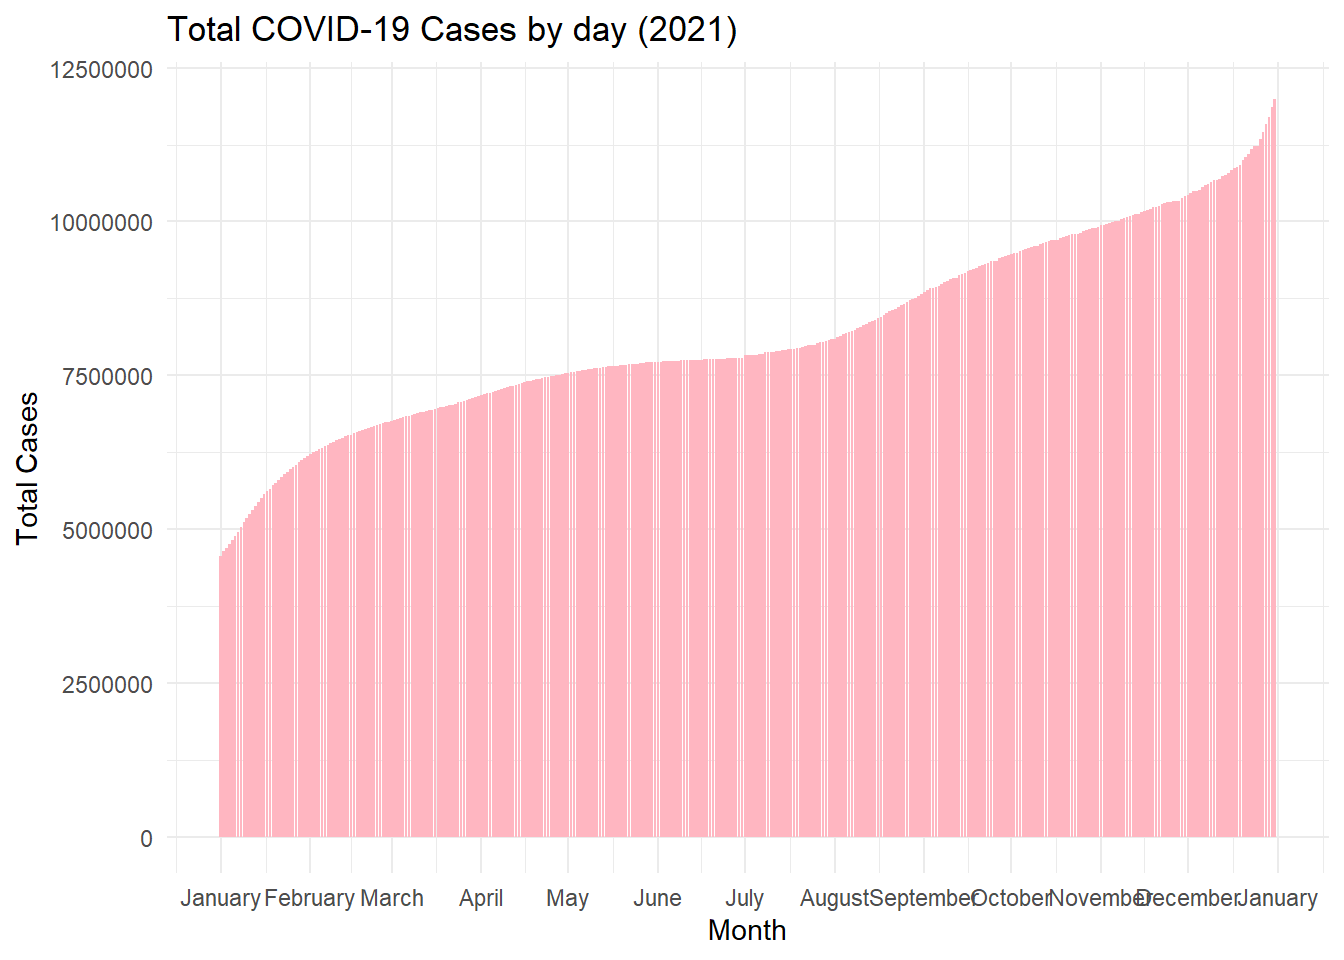
\includegraphics{Analyzing_Covid_Data_files/figure-latex/unnamed-chunk-8-4.pdf}

\begin{Shaded}
\begin{Highlighting}[]
\CommentTok{\# Summarize deaths for 2020 and 2021}
\NormalTok{deaths\_by\_day\_2020\_new }\OtherTok{\textless{}{-}} \FunctionTok{summarize\_by\_day}\NormalTok{(Covid2020StateFiltered, deaths)}
\NormalTok{deaths\_by\_day\_2021\_new }\OtherTok{\textless{}{-}} \FunctionTok{summarize\_by\_day}\NormalTok{(Covid2021StateFiltered, deaths)}

\CommentTok{\# Plot total deaths by day for 2020 and 2021}
\FunctionTok{plot\_daily\_totals}\NormalTok{(deaths\_by\_day\_2020\_new, }\StringTok{"Total COVID{-}19 Deaths by day (2020)"}\NormalTok{, }\StringTok{"Total Deaths"}\NormalTok{, }\StringTok{"darkblue"}\NormalTok{)}
\end{Highlighting}
\end{Shaded}

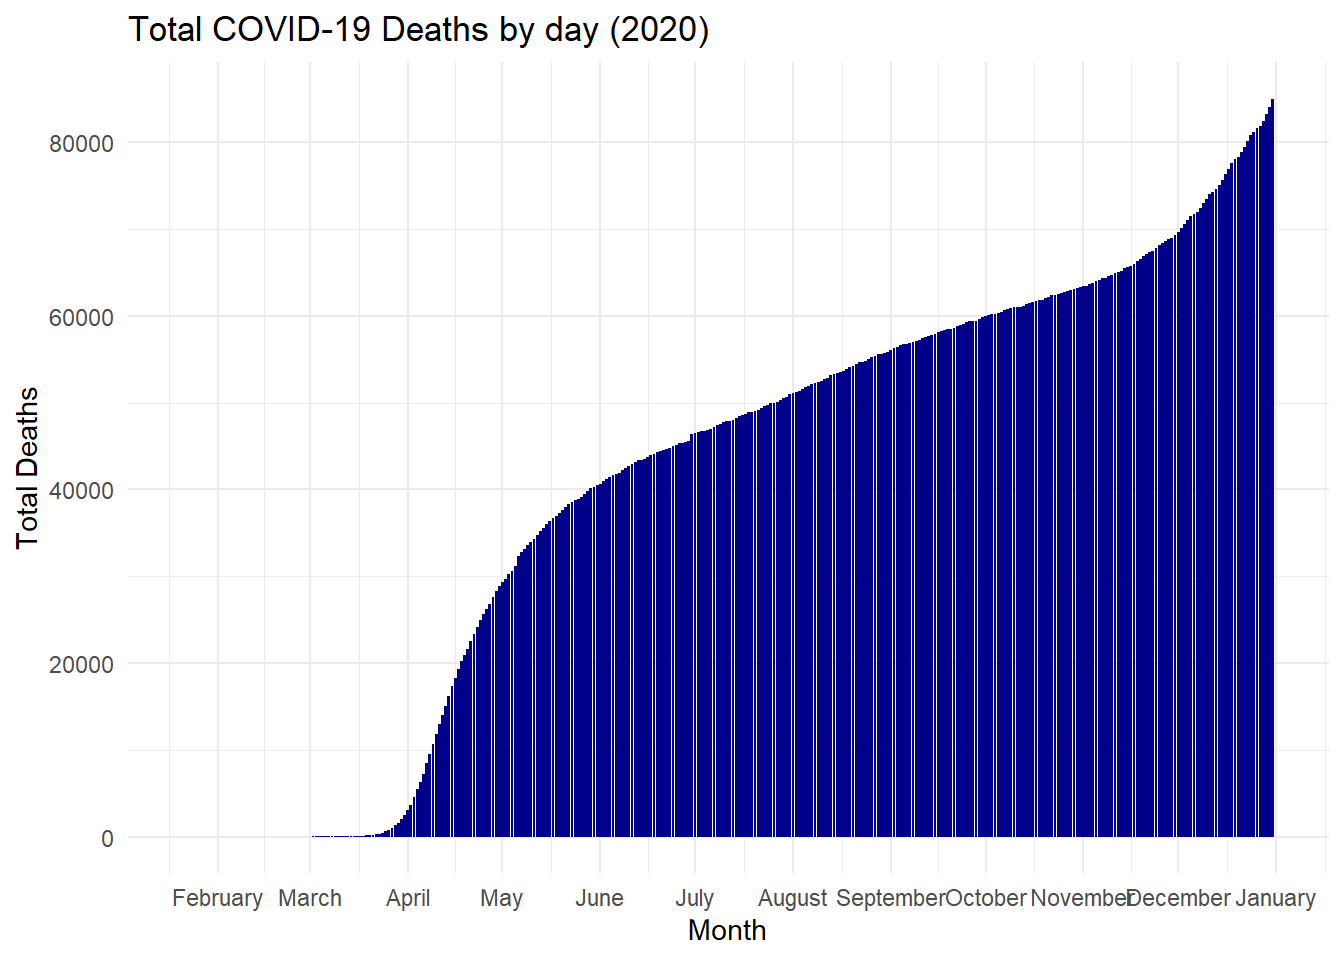
\includegraphics{Analyzing_Covid_Data_files/figure-latex/unnamed-chunk-8-5.pdf}

\begin{Shaded}
\begin{Highlighting}[]
\FunctionTok{plot\_daily\_totals}\NormalTok{(deaths\_by\_day\_2021\_new, }\StringTok{"Total COVID{-}19 Deaths by day (2021)"}\NormalTok{, }\StringTok{"Total Deaths"}\NormalTok{, }\StringTok{"darkgreen"}\NormalTok{)}
\end{Highlighting}
\end{Shaded}

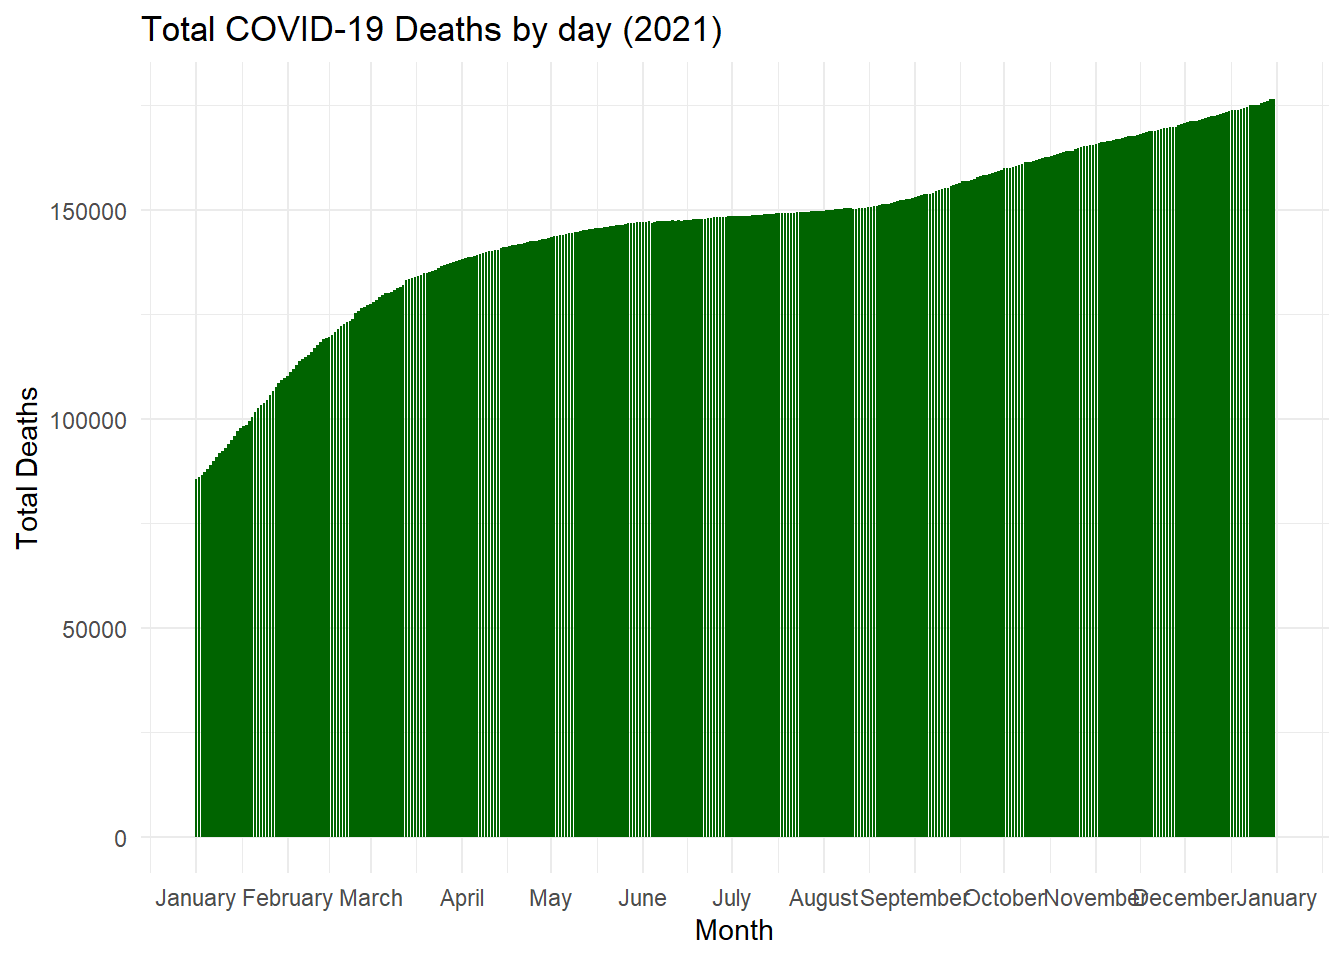
\includegraphics{Analyzing_Covid_Data_files/figure-latex/unnamed-chunk-8-6.pdf}

\begin{Shaded}
\begin{Highlighting}[]
\CommentTok{\# Filtering IQR for both cases and deaths for 2020}
\NormalTok{cases\_iqr\_2020\_new }\OtherTok{\textless{}{-}} \FunctionTok{filter\_iqr}\NormalTok{(Covid2020StateFiltered}\SpecialCharTok{$}\NormalTok{cases)}
\NormalTok{deaths\_iqr\_2020\_new }\OtherTok{\textless{}{-}} \FunctionTok{filter\_iqr}\NormalTok{(Covid2020StateFiltered}\SpecialCharTok{$}\NormalTok{deaths)}
\FunctionTok{suppressWarnings}\NormalTok{(\{}
\CommentTok{\# Plot histogram and density for cases and deaths in 2020}
\FunctionTok{print}\NormalTok{(}\FunctionTok{plot\_hist\_density}\NormalTok{(cases\_iqr\_2020\_new, }\StringTok{"Histogram of COVID 2020 Cases with Density Overlay"}\NormalTok{, }\AttributeTok{binwidth =} \DecValTok{100}\NormalTok{))}
\FunctionTok{print}\NormalTok{(}\FunctionTok{plot\_hist\_density}\NormalTok{(deaths\_iqr\_2020\_new, }\StringTok{"Histogram of COVID 2020 Deaths with Density Overlay"}\NormalTok{, }\AttributeTok{binwidth =} \DecValTok{1}\NormalTok{))}

\CommentTok{\# Remove non{-}positive values and fit gamma distribution for 2020 cases and deaths}
\NormalTok{cases\_iqr\_2020\_new }\OtherTok{\textless{}{-}}\NormalTok{ cases\_iqr\_2020\_new[cases\_iqr\_2020\_new }\SpecialCharTok{\textgreater{}} \DecValTok{0}\NormalTok{]}
\NormalTok{deaths\_iqr\_2020\_new }\OtherTok{\textless{}{-}}\NormalTok{ deaths\_iqr\_2020\_new[deaths\_iqr\_2020\_new }\SpecialCharTok{\textgreater{}} \DecValTok{0} \SpecialCharTok{\&} \SpecialCharTok{!}\FunctionTok{is.na}\NormalTok{(deaths\_iqr\_2020\_new)]}

\CommentTok{\#plot\_gamma\_fit(cases\_iqr\_2020\_new, "Histogram of COVID Cases (IQR Filtered) with Gamma Distribution Overlay (2020)", binwidth = 10)}
\FunctionTok{print}\NormalTok{(}\FunctionTok{plot\_gamma\_fit}\NormalTok{(deaths\_iqr\_2020\_new, }\StringTok{"Histogram of COVID Deaths (IQR Filtered) with Gamma Distribution Overlay (2020)"}\NormalTok{, }\AttributeTok{binwidth =} \DecValTok{1}\NormalTok{))}

\CommentTok{\# Repeat for 2021}
\NormalTok{cases\_iqr\_2021\_new }\OtherTok{\textless{}{-}} \FunctionTok{filter\_iqr}\NormalTok{(Covid2021}\SpecialCharTok{$}\NormalTok{cases)}
\NormalTok{deaths\_iqr\_2021\_new }\OtherTok{\textless{}{-}} \FunctionTok{filter\_iqr}\NormalTok{(Covid2021}\SpecialCharTok{$}\NormalTok{deaths)}

\CommentTok{\# Plot histogram and density for cases and deaths in 2021}
\FunctionTok{print}\NormalTok{(}\FunctionTok{plot\_hist\_density}\NormalTok{(cases\_iqr\_2021\_new, }\StringTok{"Histogram of COVID 2021 Cases with Density Overlay"}\NormalTok{, }\AttributeTok{binwidth =} \DecValTok{100}\NormalTok{))}
\FunctionTok{print}\NormalTok{(}\FunctionTok{plot\_hist\_density}\NormalTok{(deaths\_iqr\_2021\_new, }\StringTok{"Histogram of COVID 2021 Deaths with Density Overlay"}\NormalTok{, }\AttributeTok{binwidth =} \DecValTok{10}\NormalTok{))}

\CommentTok{\# Remove non{-}positive values and fit gamma distribution for 2021 cases and deaths}
\NormalTok{cases\_iqr\_2021\_new }\OtherTok{\textless{}{-}}\NormalTok{ cases\_iqr\_2021\_new[cases\_iqr\_2021\_new }\SpecialCharTok{\textgreater{}} \DecValTok{0} \SpecialCharTok{\&} \SpecialCharTok{!}\FunctionTok{is.na}\NormalTok{(cases\_iqr\_2021\_new) }\SpecialCharTok{\&} \FunctionTok{is.finite}\NormalTok{(cases\_iqr\_2021\_new)]}
\NormalTok{deaths\_iqr\_2021\_new }\OtherTok{\textless{}{-}}\NormalTok{ deaths\_iqr\_2021\_new[deaths\_iqr\_2021\_new }\SpecialCharTok{\textgreater{}} \DecValTok{0} \SpecialCharTok{\&} \SpecialCharTok{!}\FunctionTok{is.na}\NormalTok{(deaths\_iqr\_2021\_new) }\SpecialCharTok{\&} \FunctionTok{is.finite}\NormalTok{(deaths\_iqr\_2021\_new)]}

\CommentTok{\#plot\_gamma\_fit(cases\_iqr\_2021\_new, "Histogram of COVID Cases (IQR Filtered) with Gamma Distribution Overlay (2021)", binwidth = 100)}
\FunctionTok{print}\NormalTok{(}\FunctionTok{plot\_gamma\_fit}\NormalTok{(deaths\_iqr\_2021\_new, }\StringTok{"Histogram of COVID Deaths (IQR Filtered) with Gamma Distribution Overlay (2021)"}\NormalTok{, }\AttributeTok{binwidth =} \DecValTok{1}\NormalTok{))}

\CommentTok{\# Plot ECDF for 2020 Cases and Deaths}
\FunctionTok{print}\NormalTok{(}\FunctionTok{plot\_ecdf}\NormalTok{(cases\_by\_day\_2020\_new}\SpecialCharTok{$}\NormalTok{total, }\StringTok{"ECDF of COVID 2020 Cases"}\NormalTok{, }\StringTok{"Cases"}\NormalTok{))}
\FunctionTok{print}\NormalTok{(}\FunctionTok{plot\_ecdf}\NormalTok{(deaths\_by\_day\_2020\_new}\SpecialCharTok{$}\NormalTok{total, }\StringTok{"ECDF of COVID 2020 Deaths"}\NormalTok{, }\StringTok{"Deaths"}\NormalTok{))}

\CommentTok{\# Plot ECDF for 2021 Cases and Deaths}
\FunctionTok{print}\NormalTok{(}\FunctionTok{plot\_ecdf}\NormalTok{(cases\_by\_day\_2021\_new}\SpecialCharTok{$}\NormalTok{total, }\StringTok{"ECDF of COVID 2021 Cases"}\NormalTok{, }\StringTok{"Cases"}\NormalTok{))}
\FunctionTok{print}\NormalTok{(}\FunctionTok{plot\_ecdf}\NormalTok{(deaths\_by\_day\_2021\_new}\SpecialCharTok{$}\NormalTok{total, }\StringTok{"ECDF of COVID 2021 Deaths"}\NormalTok{, }\StringTok{"Deaths"}\NormalTok{))}

\CommentTok{\# Q{-}Q Plot against Gamma distribution for 2020 Cases and Deaths}
\CommentTok{\#print(plot\_qq\_gamma(cases\_iqr\_2020\_new, "Q{-}Q Plot of COVID 2020 Cases Against Fitted Gamma Distribution"))}
\FunctionTok{print}\NormalTok{(}\FunctionTok{plot\_qq\_gamma}\NormalTok{(deaths\_iqr\_2020\_new, }\StringTok{"Q{-}Q Plot of COVID 2020 Deaths Against Fitted Gamma Distribution"}\NormalTok{))}

\CommentTok{\# Q{-}Q Plot against Gamma distribution for 2021 Cases and Deaths}
\CommentTok{\#print(plot\_qq\_gamma(cases\_iqr\_2021\_new, "Q{-}Q Plot of COVID 2021 Cases Against Fitted Gamma Distribution"))}
\FunctionTok{print}\NormalTok{(}\FunctionTok{plot\_qq\_gamma}\NormalTok{(deaths\_iqr\_2021\_new, }\StringTok{"Q{-}Q Plot of COVID 2021 Deaths Against Fitted Gamma Distribution"}\NormalTok{))}
\NormalTok{\})}
\end{Highlighting}
\end{Shaded}

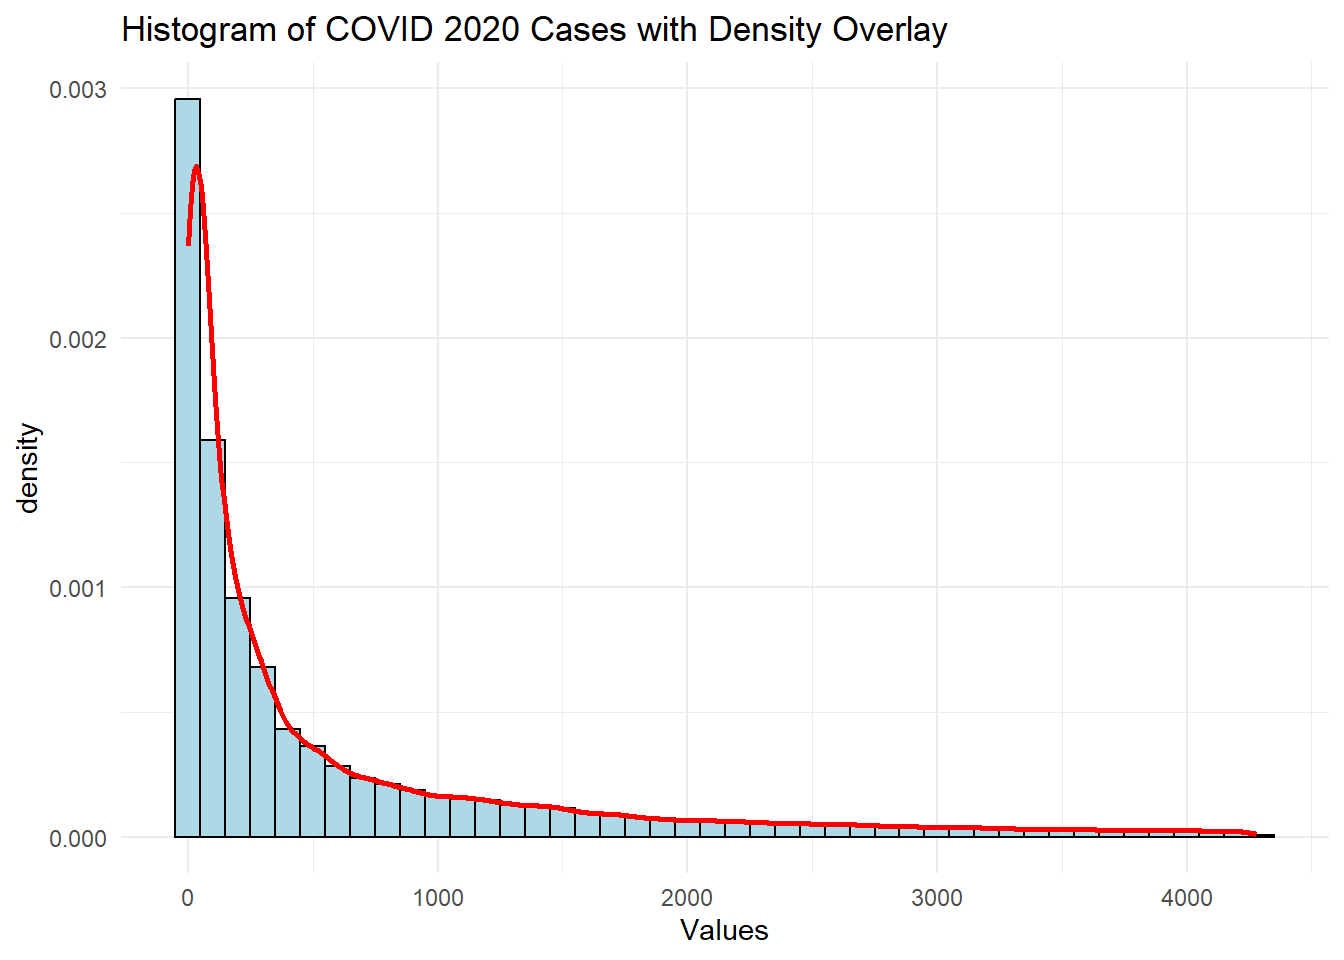
\includegraphics{Analyzing_Covid_Data_files/figure-latex/unnamed-chunk-8-7.pdf}
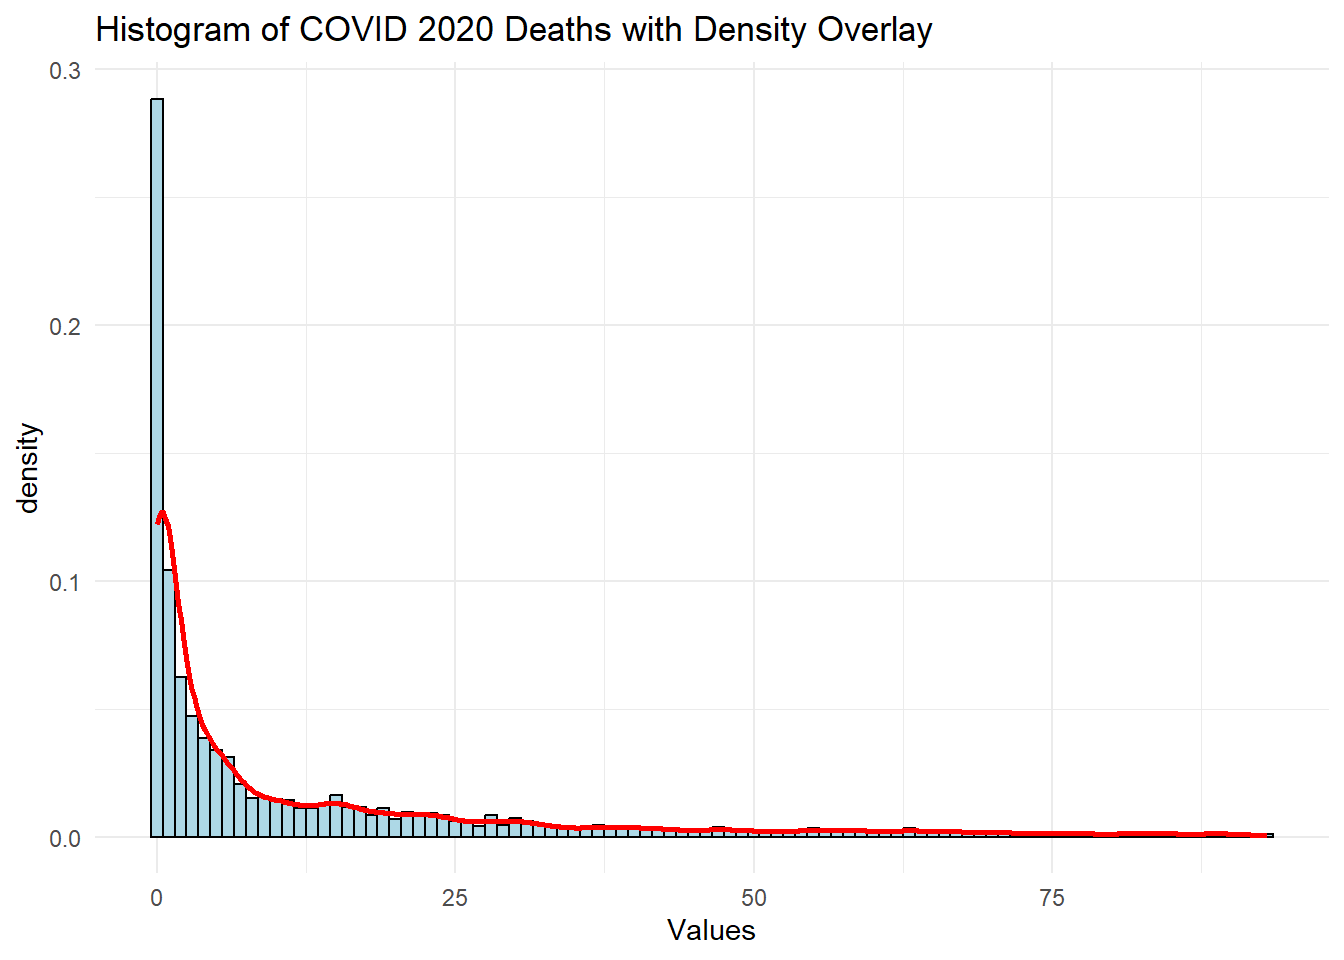
\includegraphics{Analyzing_Covid_Data_files/figure-latex/unnamed-chunk-8-8.pdf}
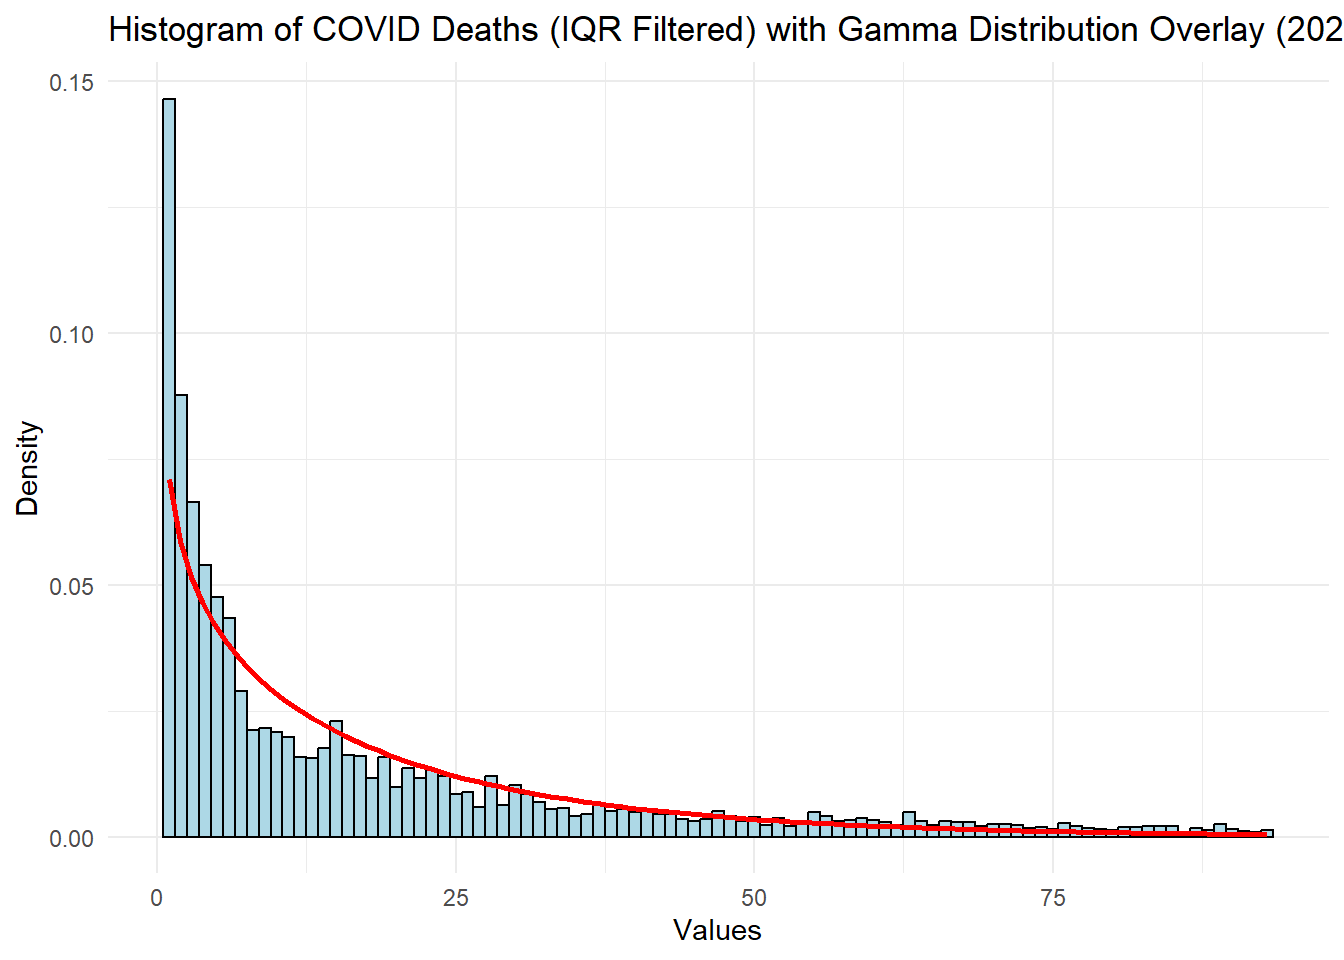
\includegraphics{Analyzing_Covid_Data_files/figure-latex/unnamed-chunk-8-9.pdf}
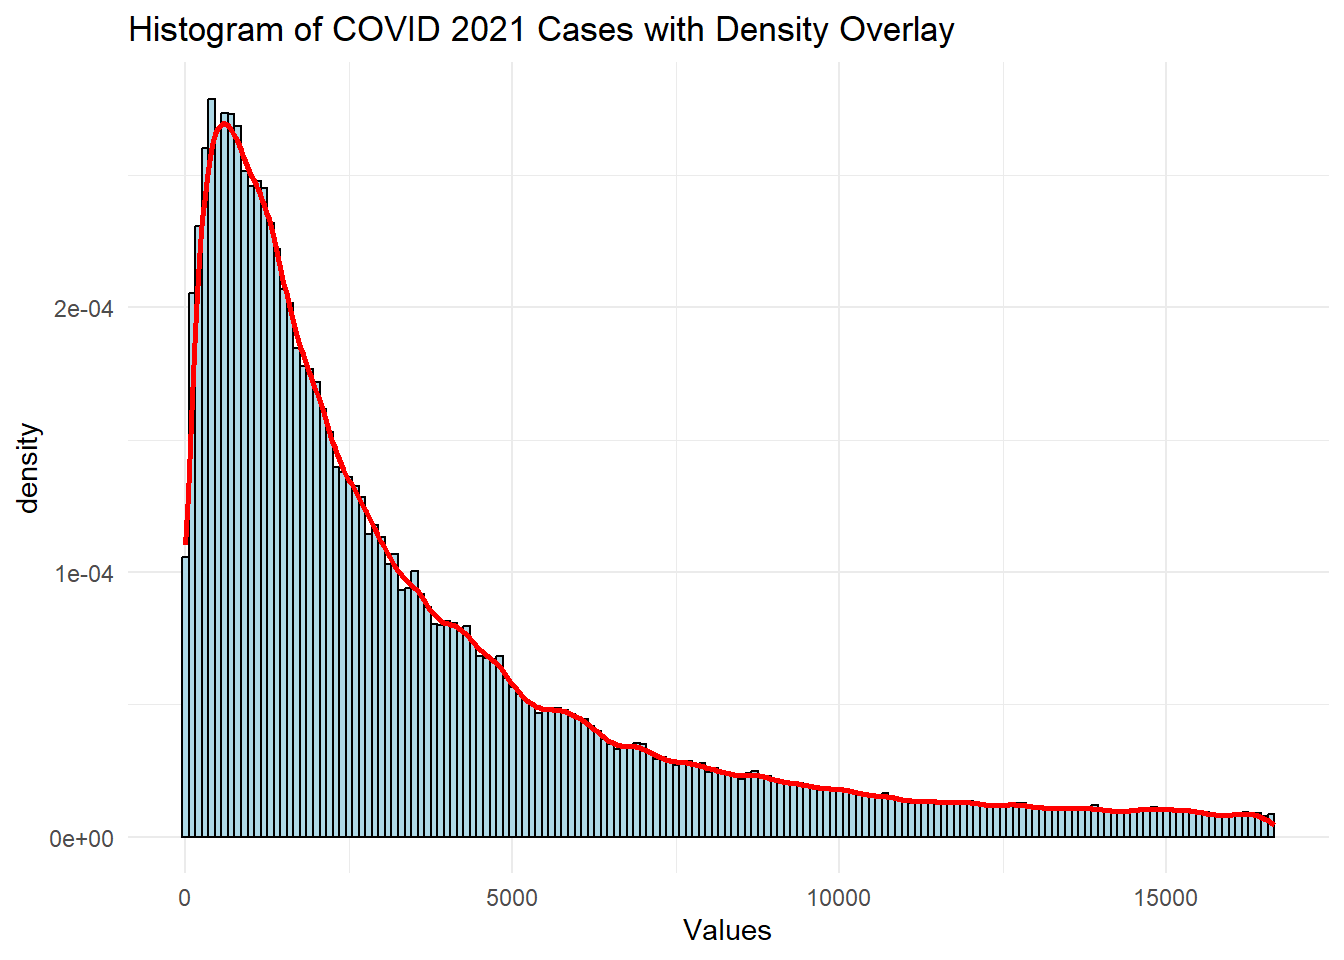
\includegraphics{Analyzing_Covid_Data_files/figure-latex/unnamed-chunk-8-10.pdf}
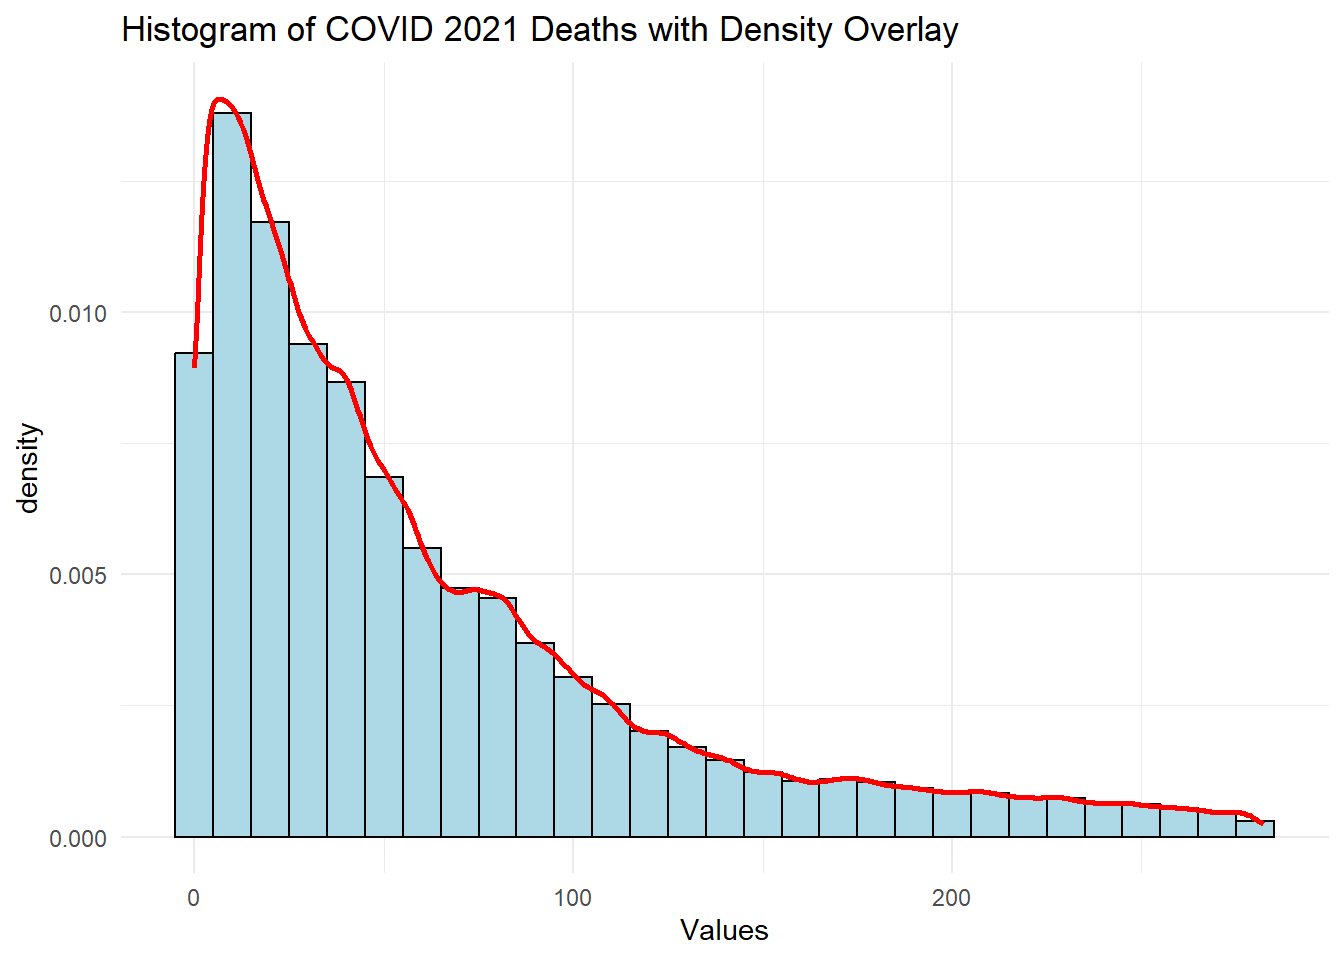
\includegraphics{Analyzing_Covid_Data_files/figure-latex/unnamed-chunk-8-11.pdf}
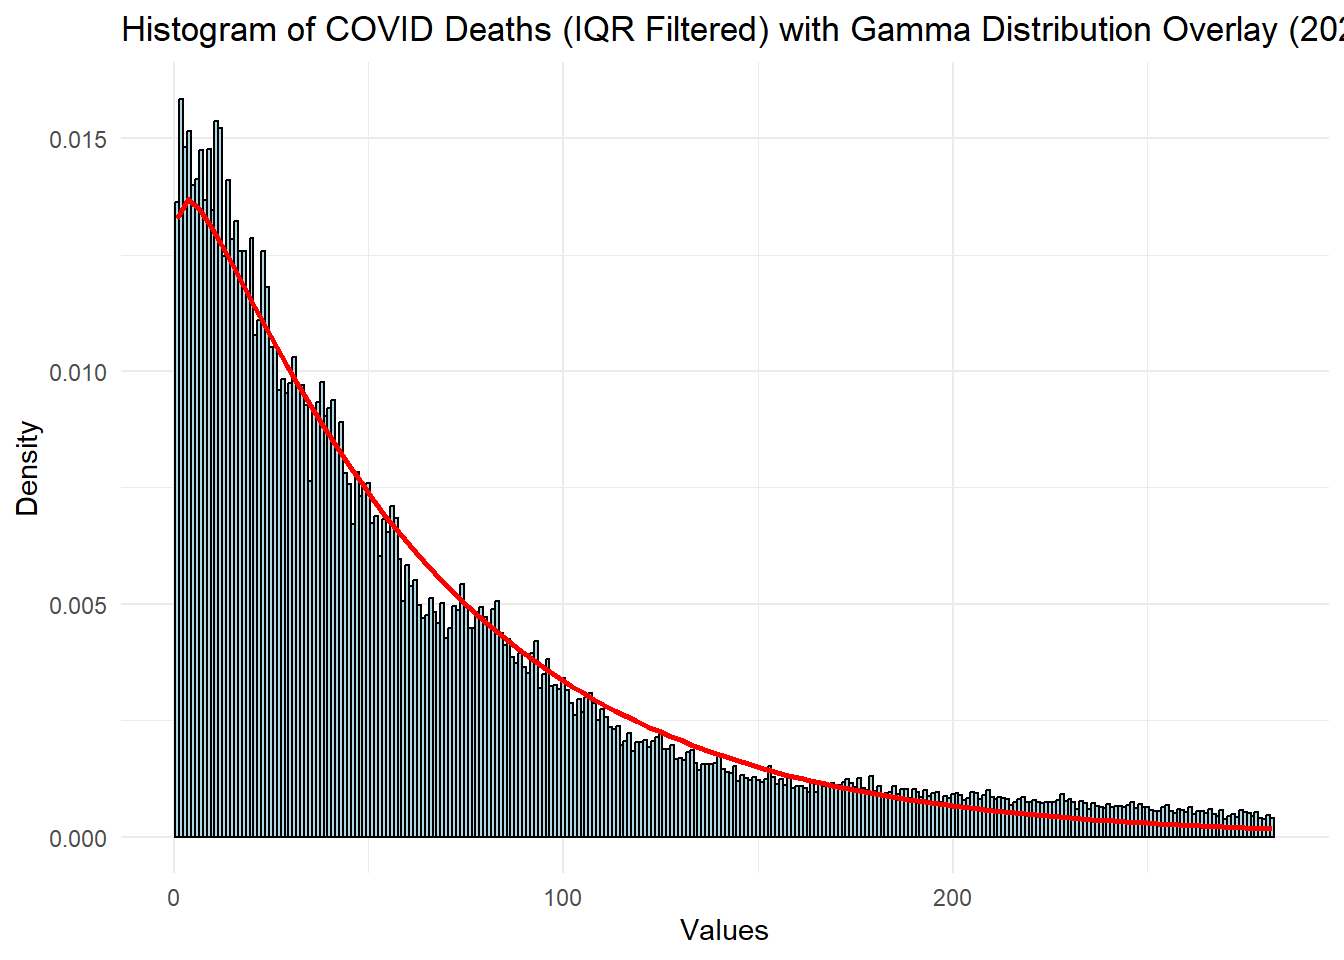
\includegraphics{Analyzing_Covid_Data_files/figure-latex/unnamed-chunk-8-12.pdf}
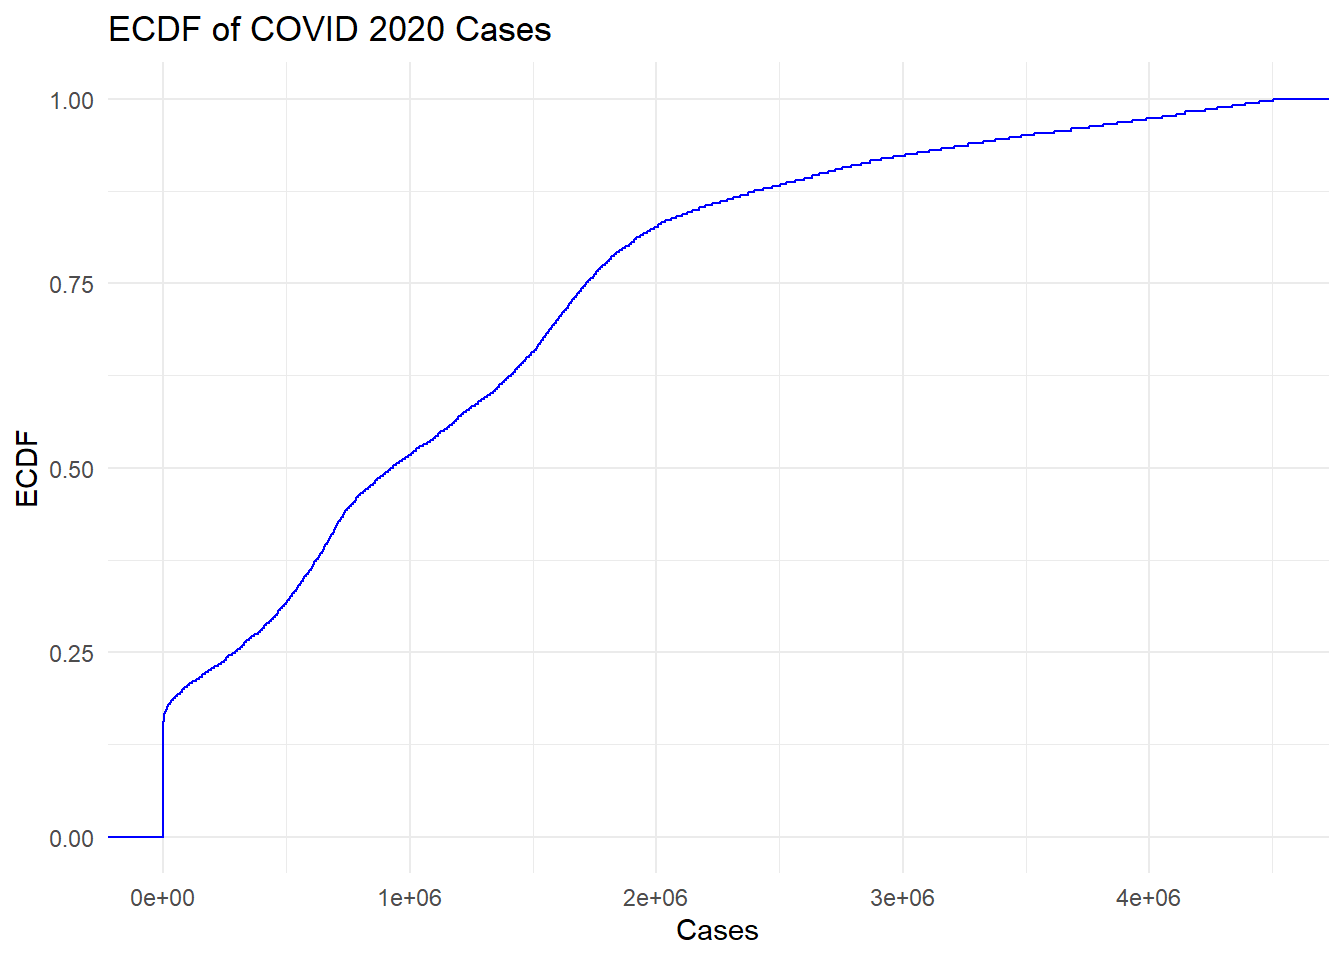
\includegraphics{Analyzing_Covid_Data_files/figure-latex/unnamed-chunk-8-13.pdf}
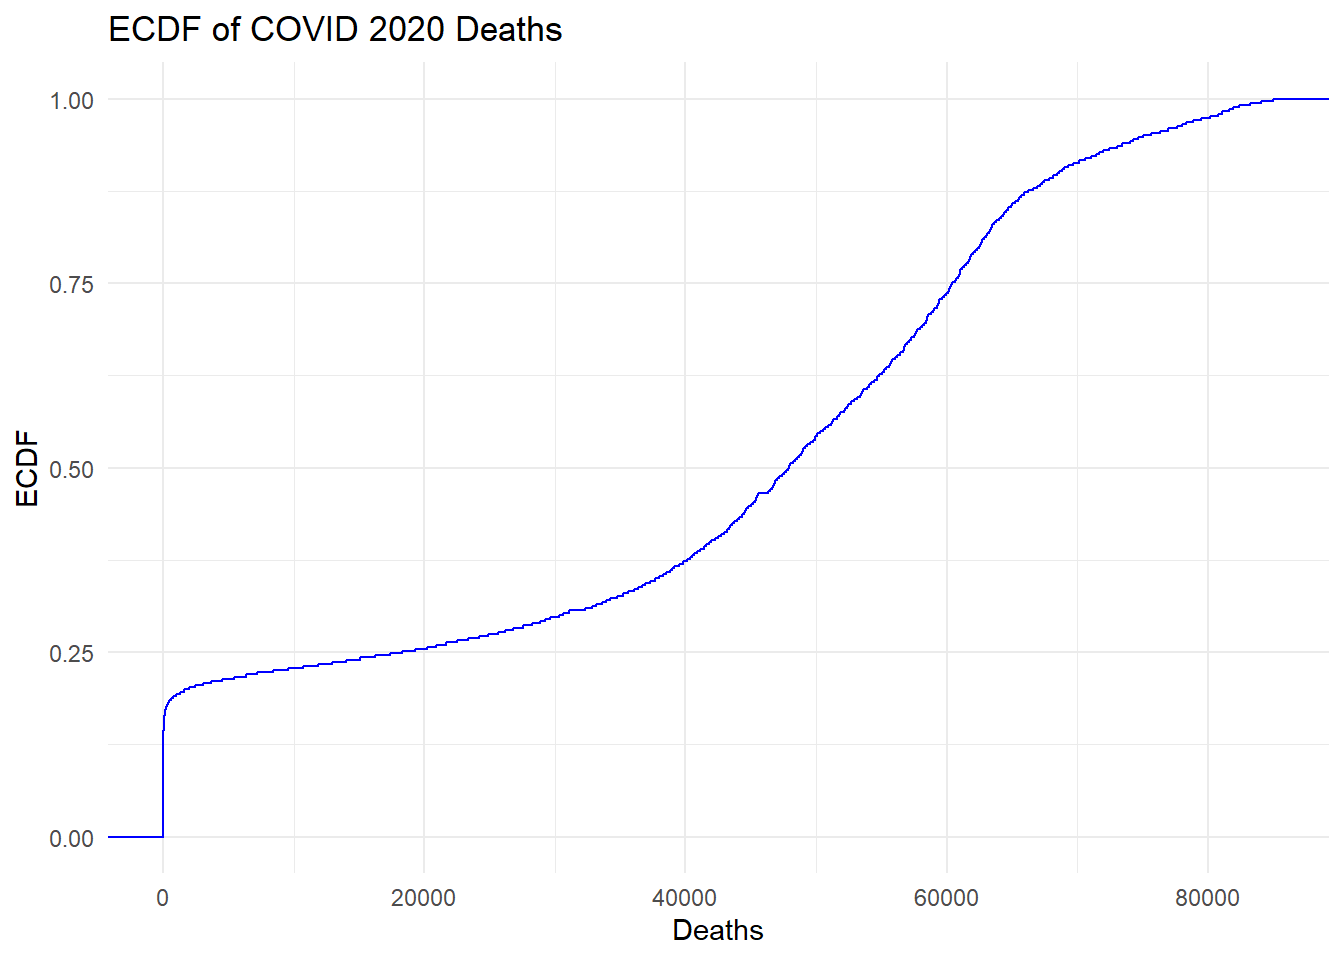
\includegraphics{Analyzing_Covid_Data_files/figure-latex/unnamed-chunk-8-14.pdf}
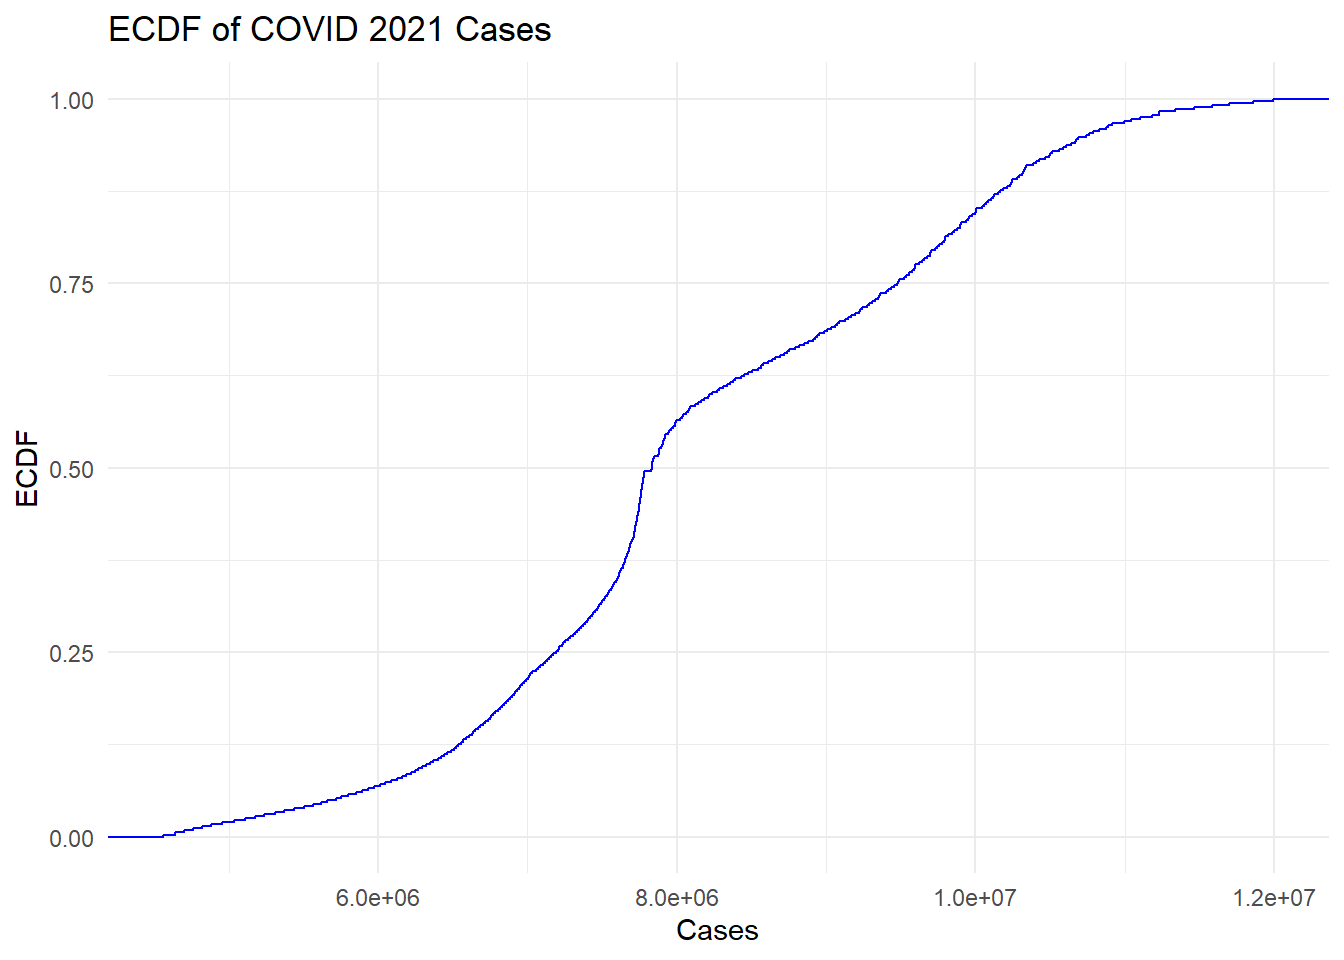
\includegraphics{Analyzing_Covid_Data_files/figure-latex/unnamed-chunk-8-15.pdf}
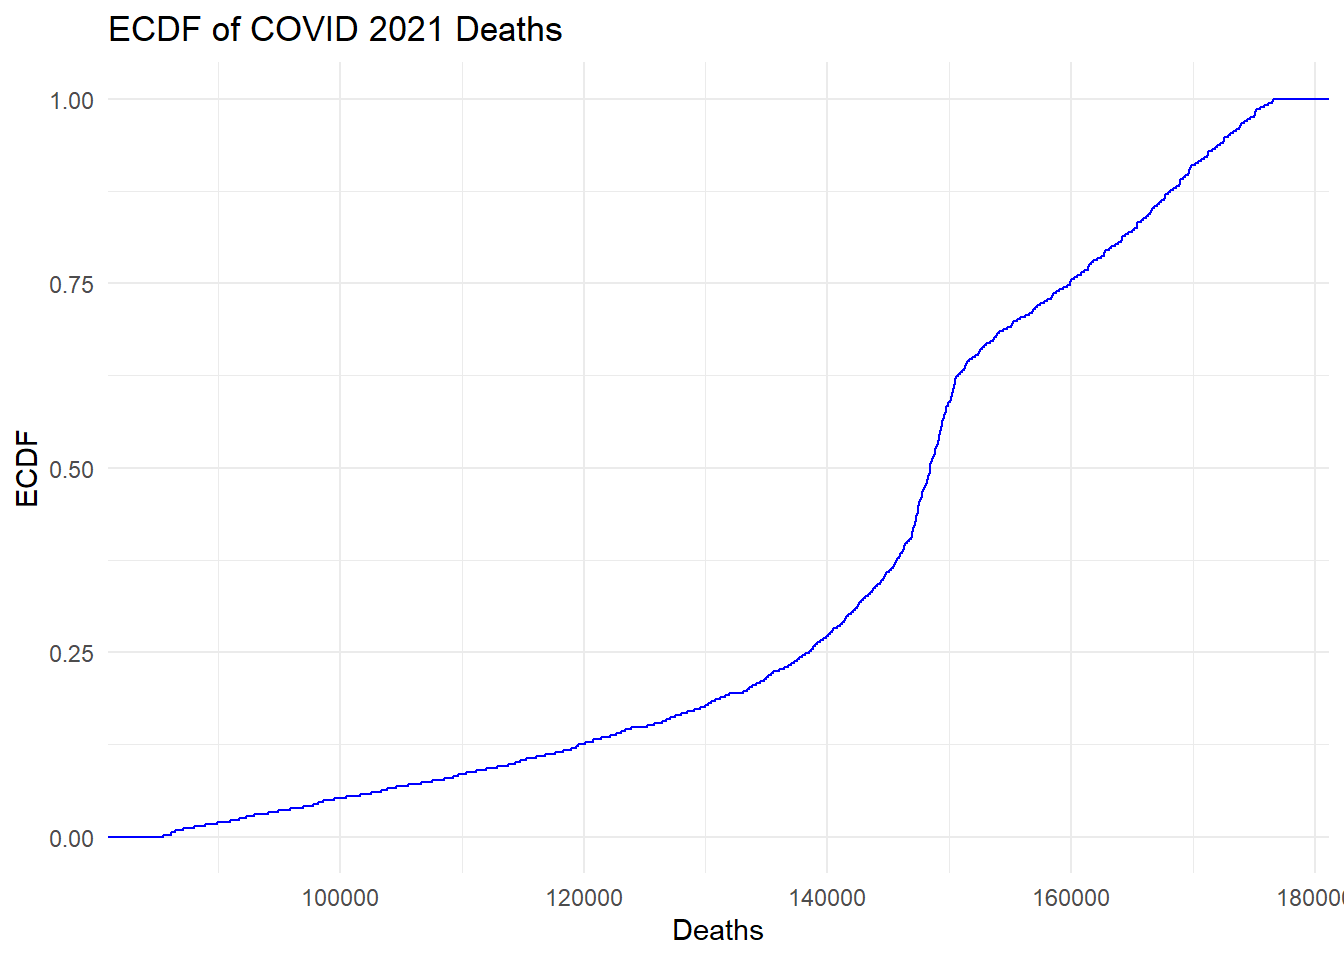
\includegraphics{Analyzing_Covid_Data_files/figure-latex/unnamed-chunk-8-16.pdf}
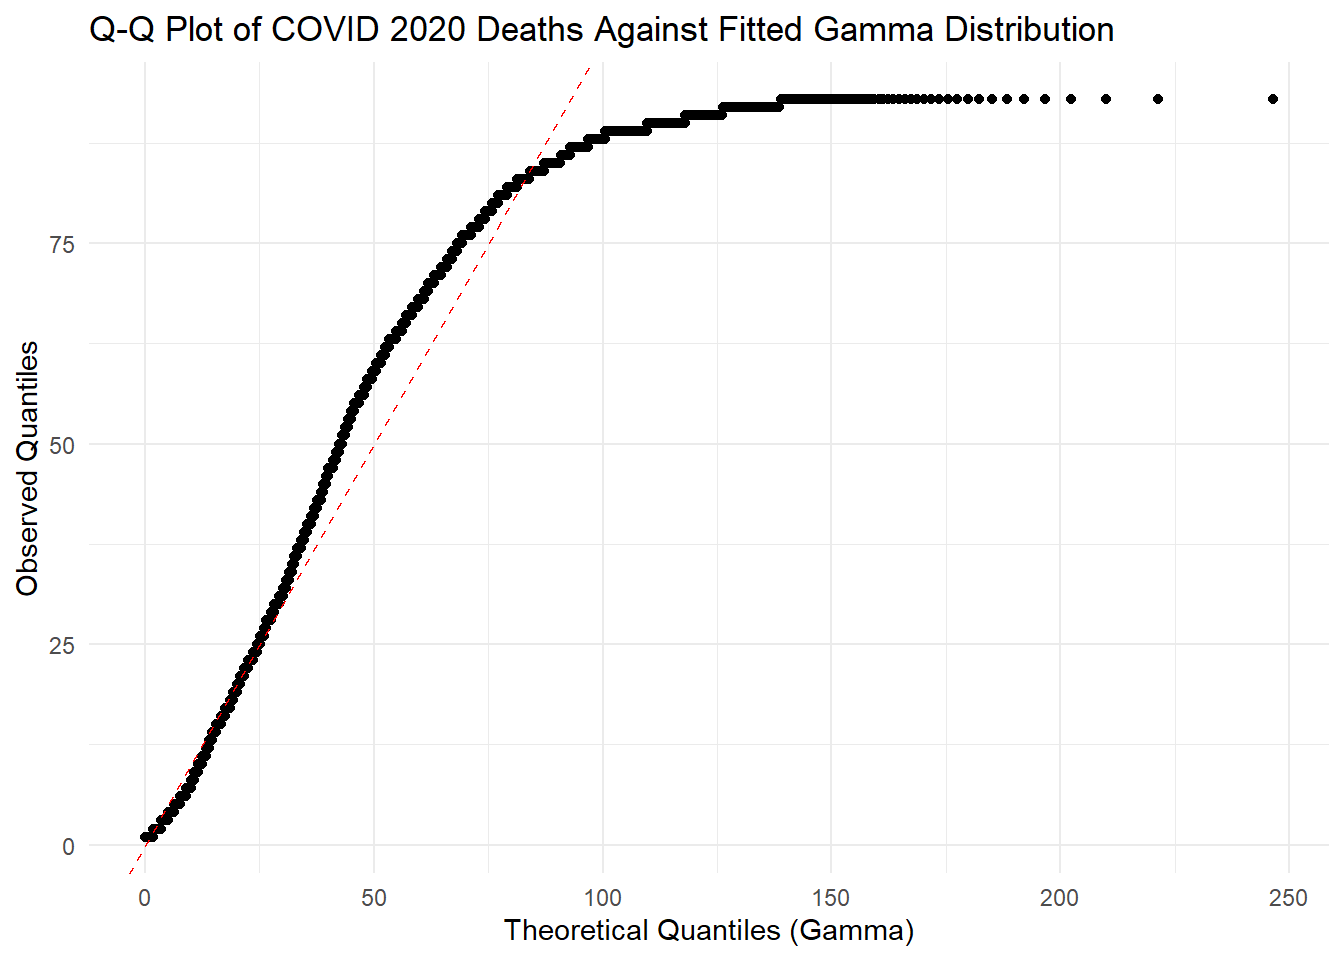
\includegraphics{Analyzing_Covid_Data_files/figure-latex/unnamed-chunk-8-17.pdf}
\includegraphics{Analyzing_Covid_Data_files/figure-latex/unnamed-chunk-8-18.pdf}

\emph{After sub-setting the data for 5 states, the graphs show a similar
trend. Since the data is cumulative, the histograms plotted for number
of cases each day and number of deaths each day shows an increasing
trend. The box plot and the summary tells us that the range of data is
very big. There are been a consistent sharp increase in the number of
deaths and number of cases in the years 2020 and 2021. The ECDF plot
explains that the number of cases was minimal in the first quarter of
2020. Even in the first half of the year 2020. But later with time the
number of cases began to rise significantly. The ECDF plot of number of
deaths also shows that in the first quarter, the number of deaths was
minimal. Then in the second quarter, the number of deaths increased
significantly.The number of deaths in the second half of 2020 increased
slowly compared to the second quarter.Again in the half half of 2021,
the number of deaths significantly. But in the second half of 2021, the
increase in number of deaths was relatively slower. The trend in the QQ
plot is similar to the original dataset.}

\end{document}
